\chapter{Systematic Uncertainties}
\label{chap:Systematics}

Different sources of systematic uncertainty contribute to the estimation of background events and modeling of the signal. The chapter is organized as follows. Theoretical uncertainties concerning signals and major backgrounds are discussed in \autoref{sec:ThUnc}. Uncertainties concerning the \emph{nonprompt} background are discussed in \autoref{sec:NonUnc}. Uncertainties concerning the modeling of the diboson processes are described in \autoref{sec:DiUnc}. Finally, other systematic uncertainties are discussed in \autoref{sec:OthUnc}.
%%%%%%%%%%%%%%%%%%%%%%%%%%%%%%%%%%%%%%%%%%%%%%%%%%%%%%%%
%%%%%%%%%%%%%%%%%%%%%%%%%%%%%%%%%%%%%%%%%%%%%%%%%%%%%%%%

\section{Theoretical Uncertainties}
\label{sec:ThUnc}

Variations on theoretical cross sections for \emph{prompt} backgrounds are introduced to cover the uncertainties in perturbative \ac{QCD} calculations. A 6$\%$ normalization uncertainty is assigned to WZ and ZZ processes~\cite{Campbell:2011bn}. A 15$\%$ normalization uncertainty is assigned to $\ttbar$W, $\ttbar$Z, and $\ttbar$H processes~\cite{Frederix:2021agh,Kulesza:2020nfh}. A 20$\%$ normalization uncertainty is assigned to tZq process, which is a conservative estimate taken from the \ac{MC} generator. A conservative 50 $\%$ normalization uncertainty is assigned to other smaller \emph{prompt} backgrounds. All normalization uncertainties are considered uncorrelated between different processes but correlated across the years. 

Uncertainties associated with the \ac{PDF} are evaluated by using 100 replicas of the NNPDF sets~\cite{NNPDF:2014otw,NNPDF:2017mvq}. The procedure described in~\cite{CMS:2012nsv} is followed. Firstly, the sum of the generator weights of each replica is normalized to the nominal sum of the generator weights. This is done before any event selection to ensure no additional normalization effect is introduced. After the previous step, the bin-by-bin variations of the \ac{BDT} templates are obtained by calculating the bin-by-bin difference of the \ac{BDT} templates when switching from nominal \ac{PDF} to each \ac{PDF} replica. Finally, \ac{PDF} uncertainty for each bin is assigned by taking the root mean square value of the 100 variations of the corresponding bin. This uncertainty is treated as uncorrelated between different processes but correlated across the years. This uncertainty is considered for all the signals and major prompt backgrounds (i.e. WZ, $\ttbar$W, $\ttbar$Z, and $\ttbar$H).

\ac{QCD} scale uncertainties are evaluated by varying the renormalization scale $\mu_\textsf{R}$ and factorization scales $\mu_\textsf{F}$ in \ac{ME}. A total of six variations are considered: varying $\mu_\textsf{R}$ by a factor of 2 and 0.5, varying $\mu_\textsf{F}$ by a factor of 2 and 0.5, and varying $\mu_\textsf{R}$ and $\mu_\textsf{F}$ simultaneously by a factor of 2 and 0.5. Similar to PDF uncertainty, the normalization effects of each variation are removed. An envelope that covers all six variations is used to represent the scale uncertainty. This uncertainty is treated as uncorrelated between different processes but correlated across the years. This uncertainty is considered for all the signals and major prompt backgrounds (i.e. WZ, $\ttbar$W, $\ttbar$Z, and $\ttbar$H).

Uncertainties associated with the \ac{PS} are evaluated by varying the renormalization scale $\mu_\textsf{R}$ in the initial and final state radiations, which effectively changes the strong coupling constant in the \ac{PS}. Similarly, $\mu_\textsf{R}$ is varied by a factor of 2 and 0.5, and the normalization effects of each variation are removed. This uncertainty is treated as uncorrelated between different processes but correlated across the years. This uncertainty is only considered for signal events.
%%%%%%%%%%%%%%%%%%%%%%%%%%%%%%%%%%%%%%%%%%%%%%%%%%%%%%%%
%%%%%%%%%%%%%%%%%%%%%%%%%%%%%%%%%%%%%%%%%%%%%%%%%%%%%%%%

\section{Nonprompt Uncertainties}
\label{sec:NonUnc}

There are several sources of uncertainties associated with the determination of the \emph{nonprompt} efficiency $f$. One of these uncertainties comes from the estimate of \emph{prompt} contamination in \ac{MR}. As is discussed in \autoref{chap:Nonprompt}, \emph{prompt} backgrounds (estimated with \ac{MC}) are subtracted from total event yields measured in data. A flat 20 $\%$ uncertainty ($\alpha$ in Equation \ref{eq:f_eq_sys}) is assigned to the event yields of the \emph{prompt} background and the resulting variation of $f$ is taken as the uncertainty.

\begin{equation}
f=\frac{n_{data}^{tag+tight}-(1+\alpha)n_{MC(prompt)}^{tag+tight}}{n_{data}^{tag+loose}-(1+\alpha)n_{MC(prompt)}^{tag+loose}}.
\label{eq:f_eq_sys}
\end{equation}  

\begin{figure}[tbh!]
 \begin{center}
 \begin{tabular}{c}
 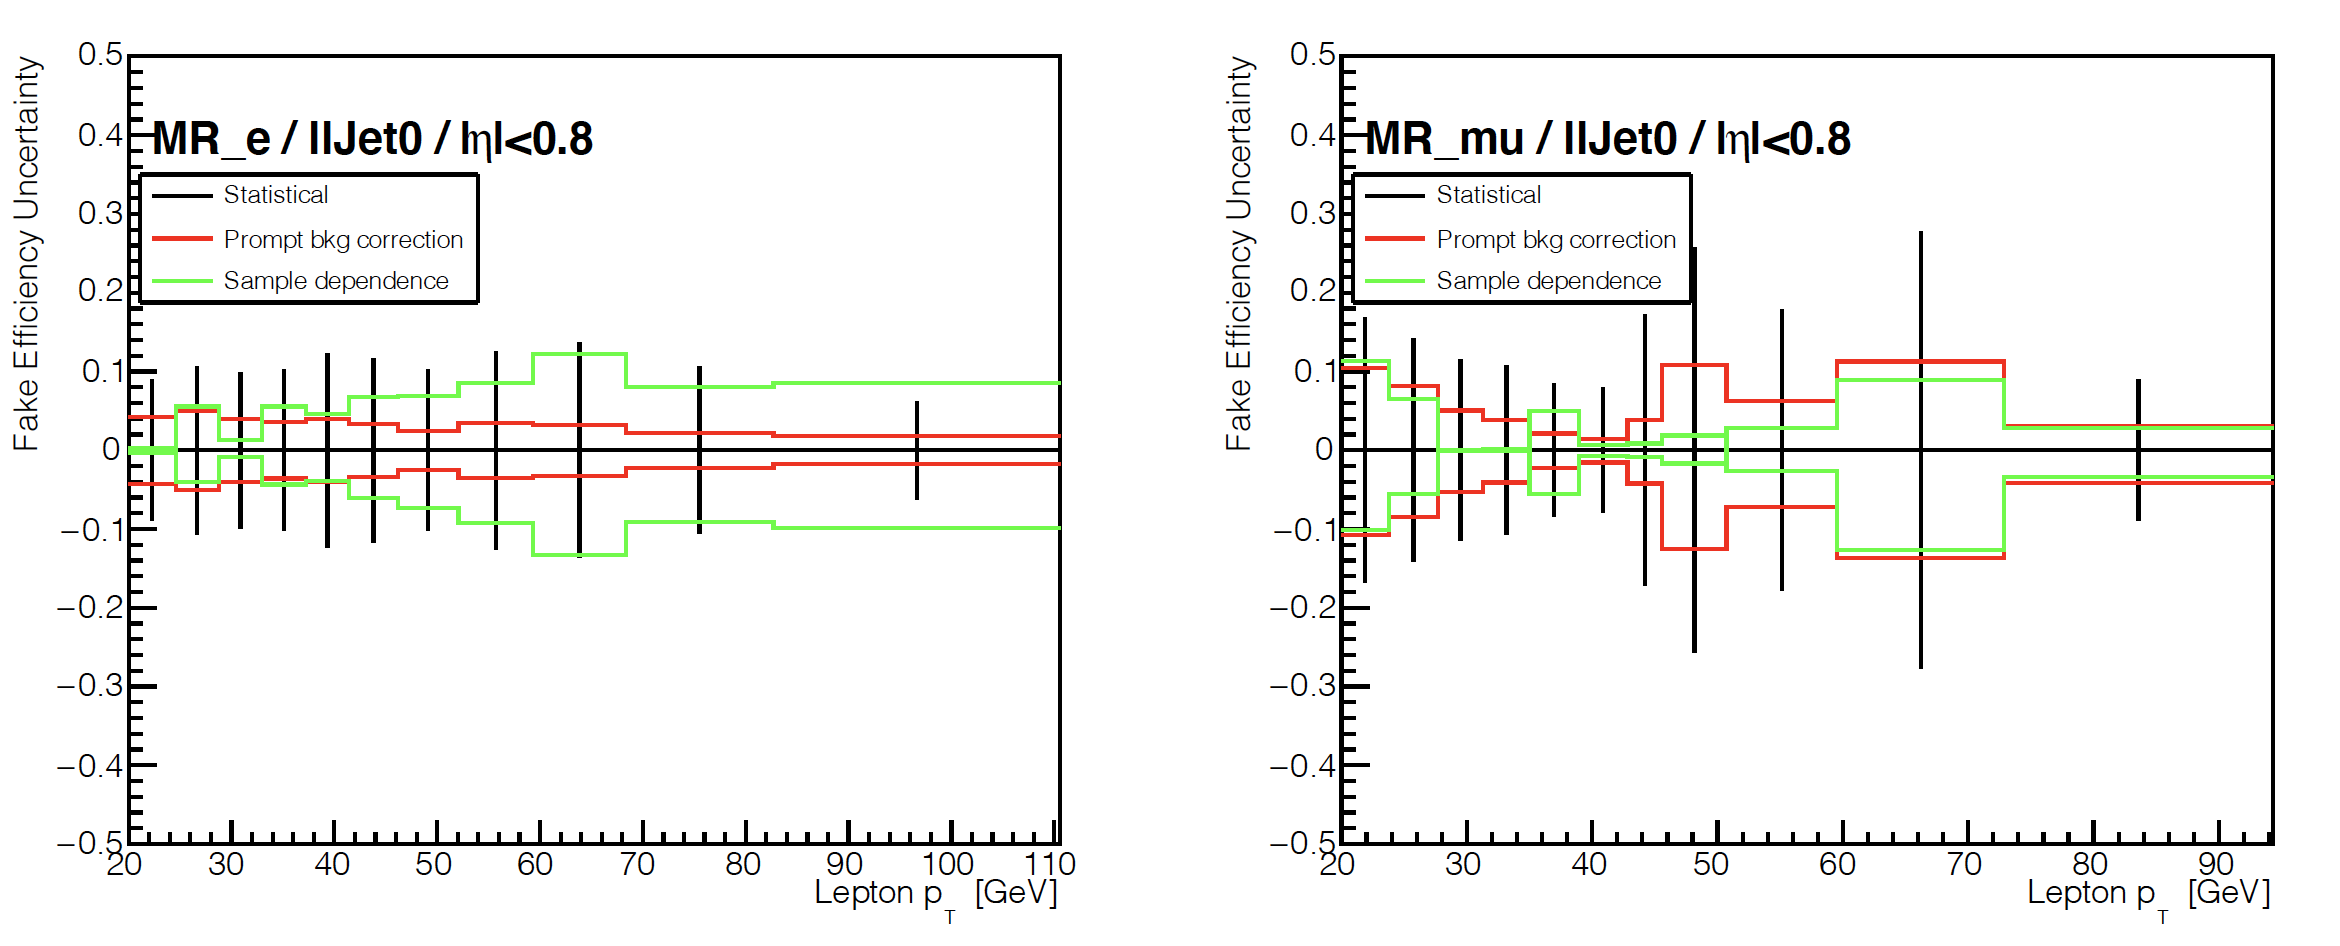
\includegraphics[width=0.99\textwidth]{figures/Part3/Systematics/MR1}
 \end{tabular}
 \caption{Comparison of different components of the uncertainties associated to the \emph{nonprompt} efficiency measured in the 2017 dataset (njet = 0 bin, $|\eta|~<$ 0.8 bin). From left to right: electron $f$ uncertainty, muon $f$ uncertainty.}
 \label{fig:f_comp1}
 \end{center}
\end{figure}

Another source of uncertainty associated with the determination of \emph{nonprompt} efficiency \emph{f} is concerned with the observation that f exhibits a flavor dependency, as is shown in Figure~\ref{fig:fake_eff}. This can happen when different physics processes enter \acp{MR} with different lepton flavor composites, which lead to differences in \emph{nonprompt} lepton behaviors. This type of uncertainty, referred to as ``sample dependence'', is estimated by introducing a variation factor $\beta$ between the proportions of same-flavor and different-flavor pairs in \ac{MR}. For example, electron \emph{f} can be calculated as (prompt background correction is ignored from the equation),

\begin{equation}
f_{\textsf{e}}=\frac{(1+\beta)n_{\textsf{e+e}}^{tag+tight}+(1-\beta)n_{\textsf{e+}\upmu}^{tag+tight}}{(1+\beta)n_{\textsf{e+e}}^{tag+loose}+(1-\beta)n_{\textsf{e+}\upmu}^{tag+loose}}.
 \label{eq:samp_dep}
\end{equation}

A 20$\%$ variation ($\beta$) is assigned the resulting variation of $f$ is taken as the uncertainty.
 
Statistical uncertainty is also considered when determining $f$. A comparison of different sources of uncertainties is shown in Figure \ref{fig:f_comp1} and Figure \ref{fig:f_comp2}. All sources of uncertainties are added in quadrature to form the final uncertainty on $f$. 

\begin{figure}[tbh!]
 \begin{center}
 \begin{tabular}{c}
 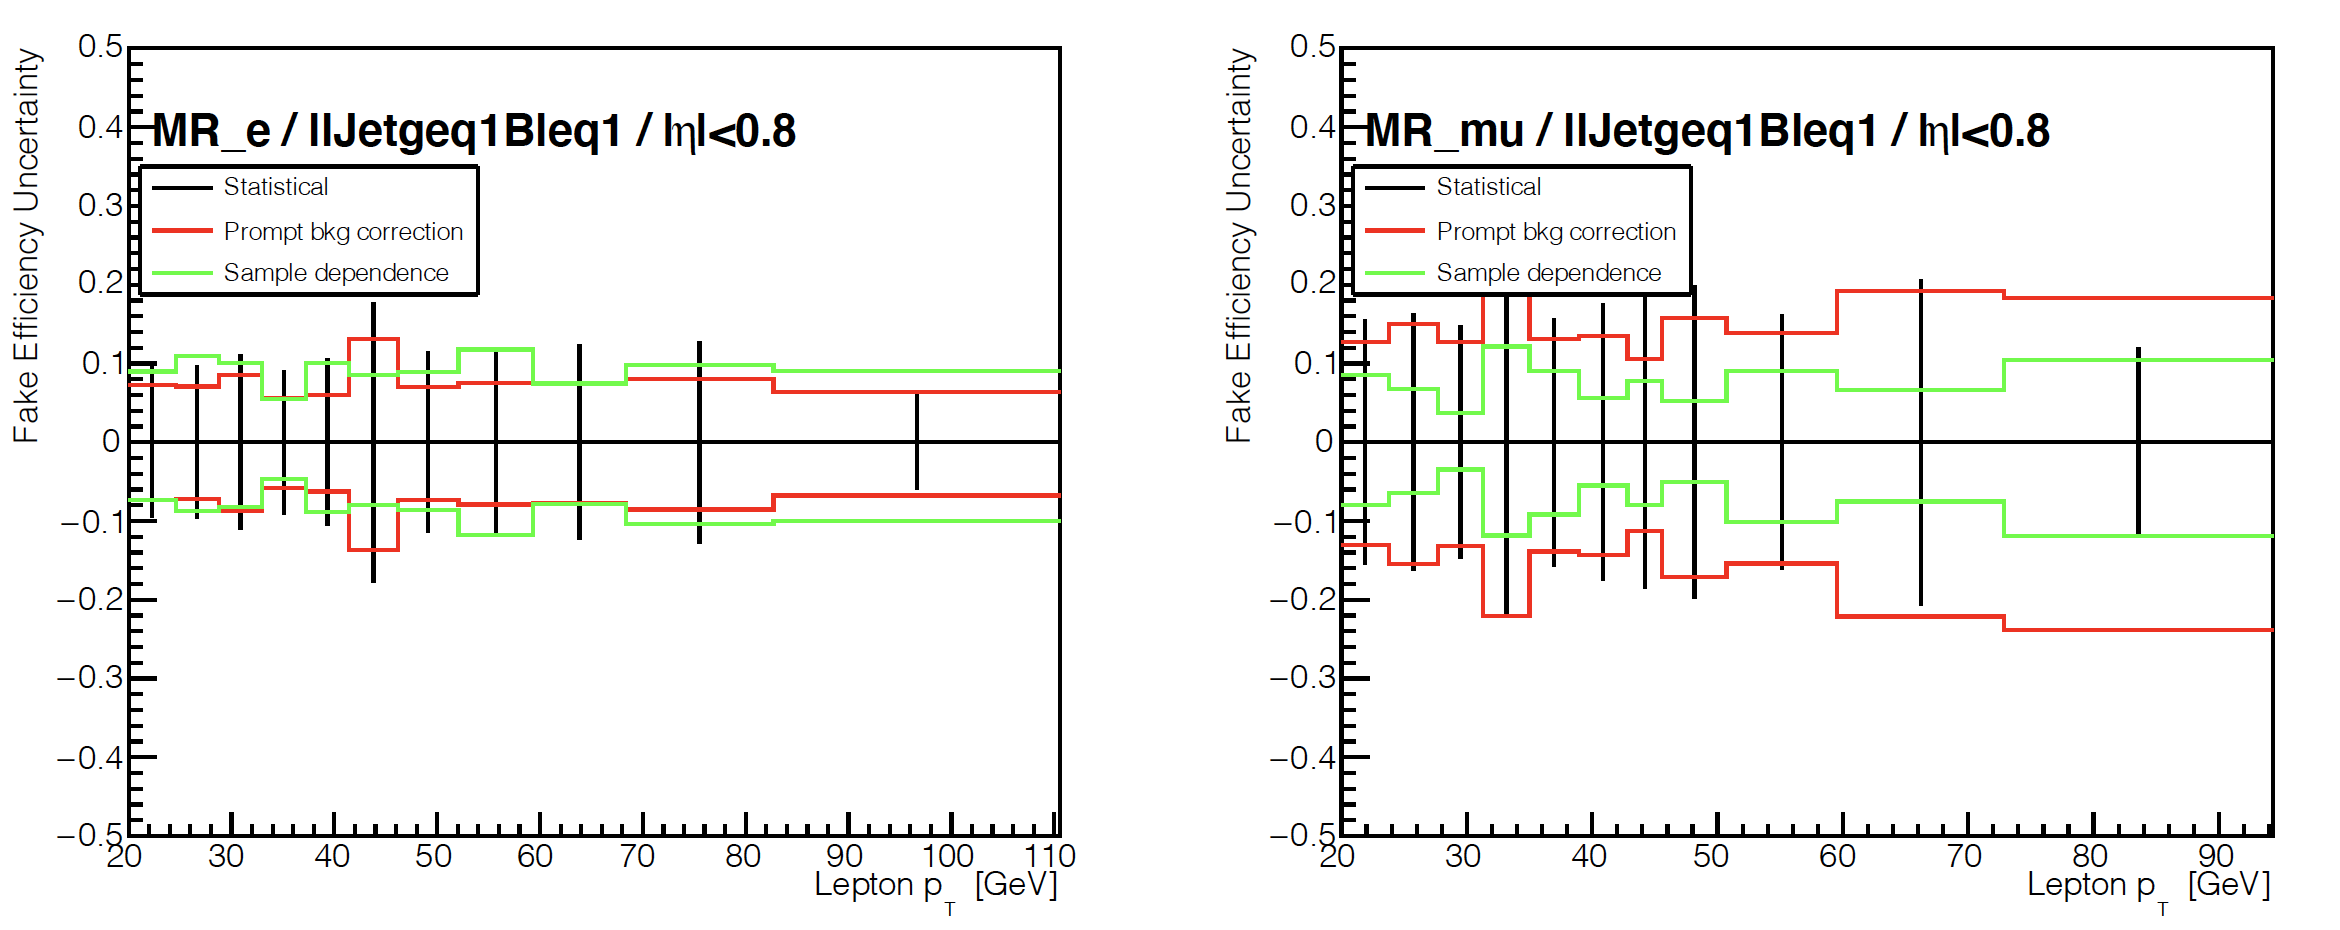
\includegraphics[width=0.99\textwidth]{figures/Part3/Systematics/MR2}
 \end{tabular}
 \caption{Comparison of different components of the uncertainties associated to the \emph{nonprompt} efficiency measured in the 2017 dataset (njet $>$ 0 bin, $|\eta|~<$ 0.8 bin). From left to right: electron $f$ uncertainty, muon $f$ uncertainty.}
 \label{fig:f_comp2}
 \end{center}
\end{figure}

Since the \emph{prompt} efficiency $r$ is measured in simulated $\ttbar$ events, \ac{MC} uncertainties described in \autoref{sec:OthUnc} are propagated to $r$ as the uncertainties. Additionally, statistical uncertainty is added in quadrature to the \ac{MC} uncertainties to form the final uncertainty on $r$.

The uncertainties associated with the \emph{prompt} efficiency are relatively small when compared to the \emph{nonprompt} efficiency uncertainties. A comparison of different sources of \emph{prompt} efficiency uncertainties is shown in Figure \ref{fig:r_comp}.

\begin{figure}[tbh!]
 \begin{center}
 \begin{tabular}{c}
 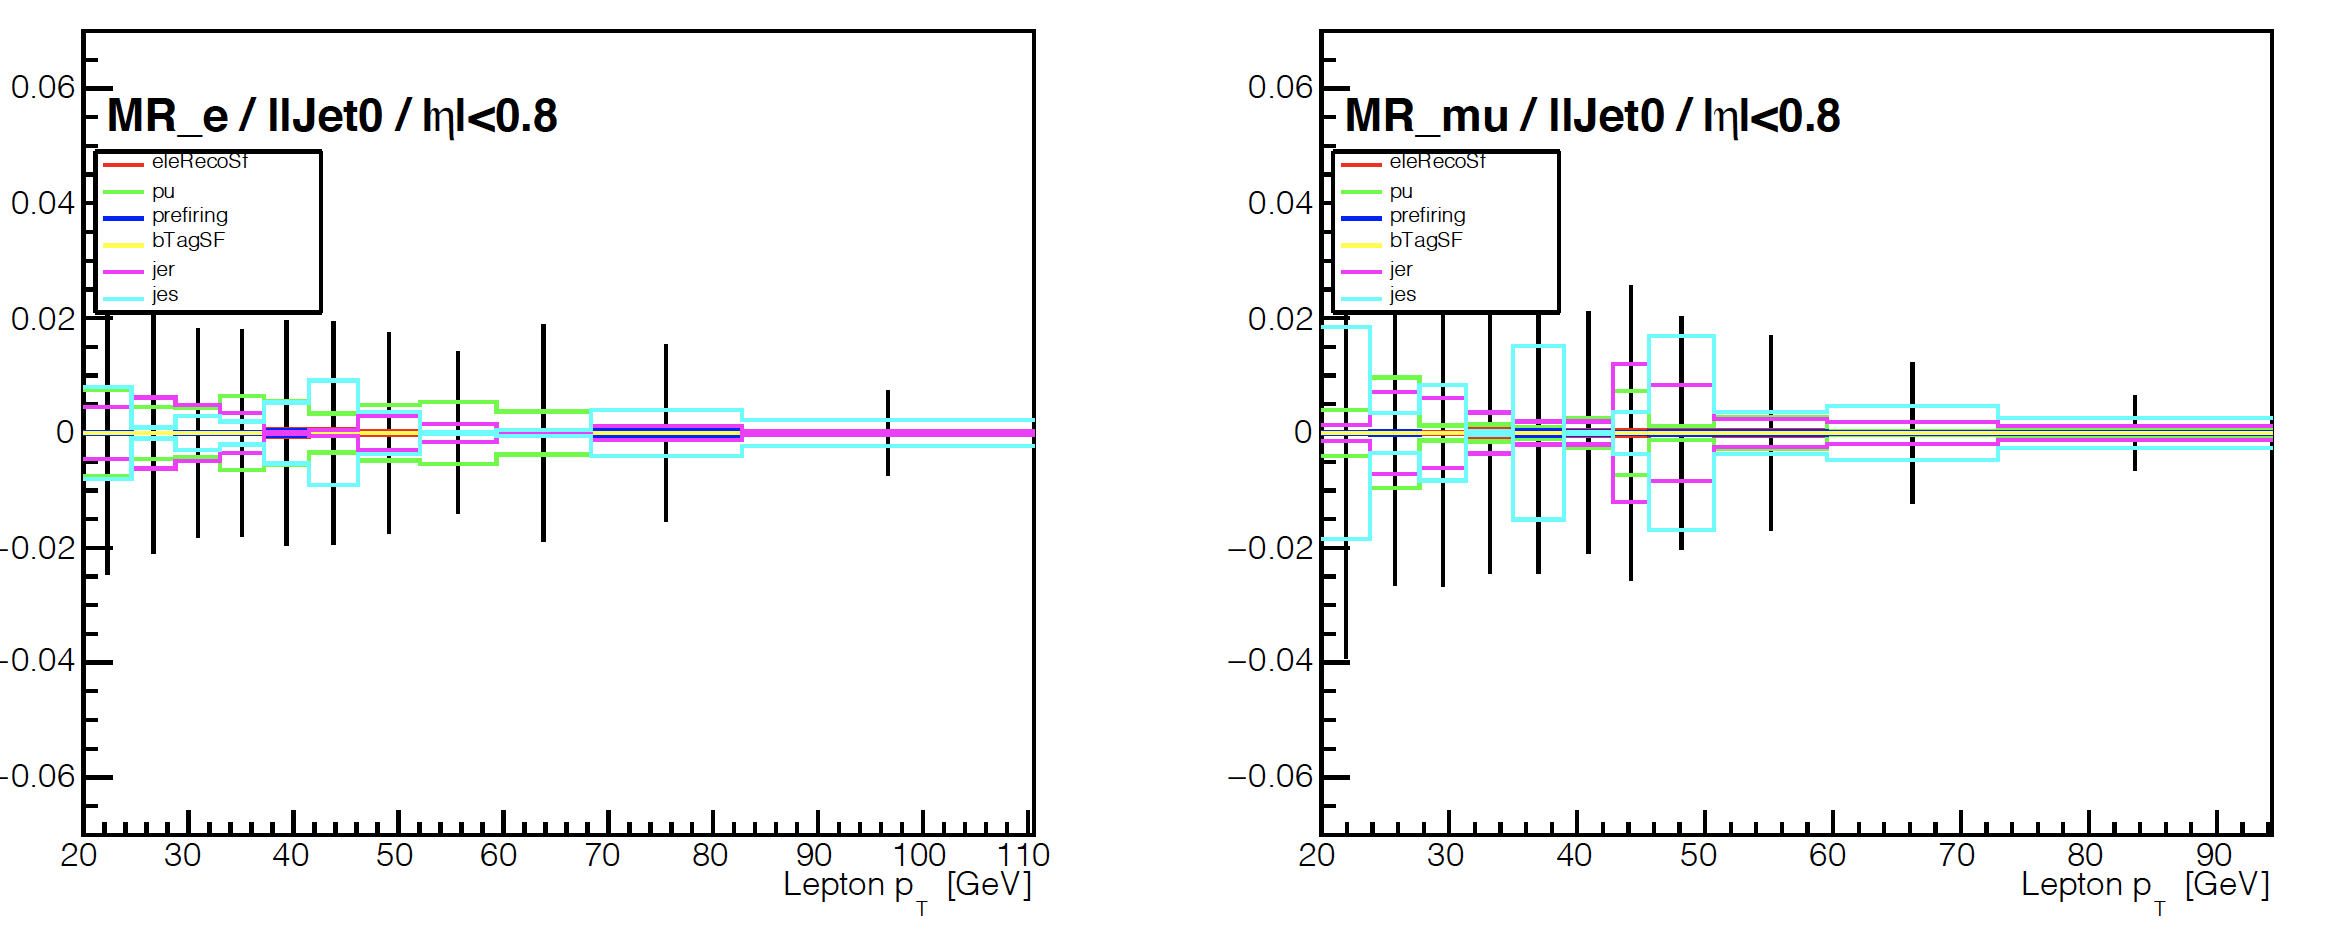
\includegraphics[width=0.99\textwidth]{figures/Part3/Systematics/MR}
 \end{tabular}
 \caption{Comparison of different components of the uncertainties associated to the \emph{prompt} efficiency measured in the 2017 dataset (njet $=$ 0 bin, $|\eta|~<$~0.8 bin). From left to right: electron $r$ uncertainty, muon $r$ uncertainty.}
 \label{fig:r_comp}
 \end{center}
\end{figure}

Uncertainties associated to $r$ and $f$ are determined separately for electron and muon. Therefore, there are four independent uncertainties: $r_{\textsf{e}}$, $r_{\upmu}$, $f_{\textsf{e}}$ and $f_{\upmu}$. 

A fifth uncertainty is considered that accounts for the potential bias caused by the way the generalized \mm~is implemented. Four out of the eight \acp{AR} that appear on the lefthand side of the Equation \ref{eq:matrix_method3} (i.e. $N^{\overline{T}TT}$, $N^{\overline{T}T\overline{T}}$, $N^{\overline{T}\overline{T}T}$, $N^{\overline{T}\overline{T}\overline{T}}$) are selected by requiring the leading lepton in $\pt$ to fail the \emph{tight} criteria described in Table~\ref{tab:looseandtight}. Effectively this means that the isolation requirement is reversed for leading lepton that enter these four \acp{AR}. Selecting the leading lepton by a loose requirement is not ideal since the leading lepton is required to match with iso-triggers. To account for this bias, a 50 $\%$ uncertainty is assigned to the $f_1$ (\emph{nonprompt} efficiency associated with the leading lepton) for events that enter these four \acp{AR}. The variation of the \emph{nonprompt} estimate due to trigger matching is largely covered by this uncertainty, as is shown in Figure~\ref{fig:MM_trigger}.

\begin{figure}[tbh!]
 \begin{center}
 \begin{tabular}{cc}
 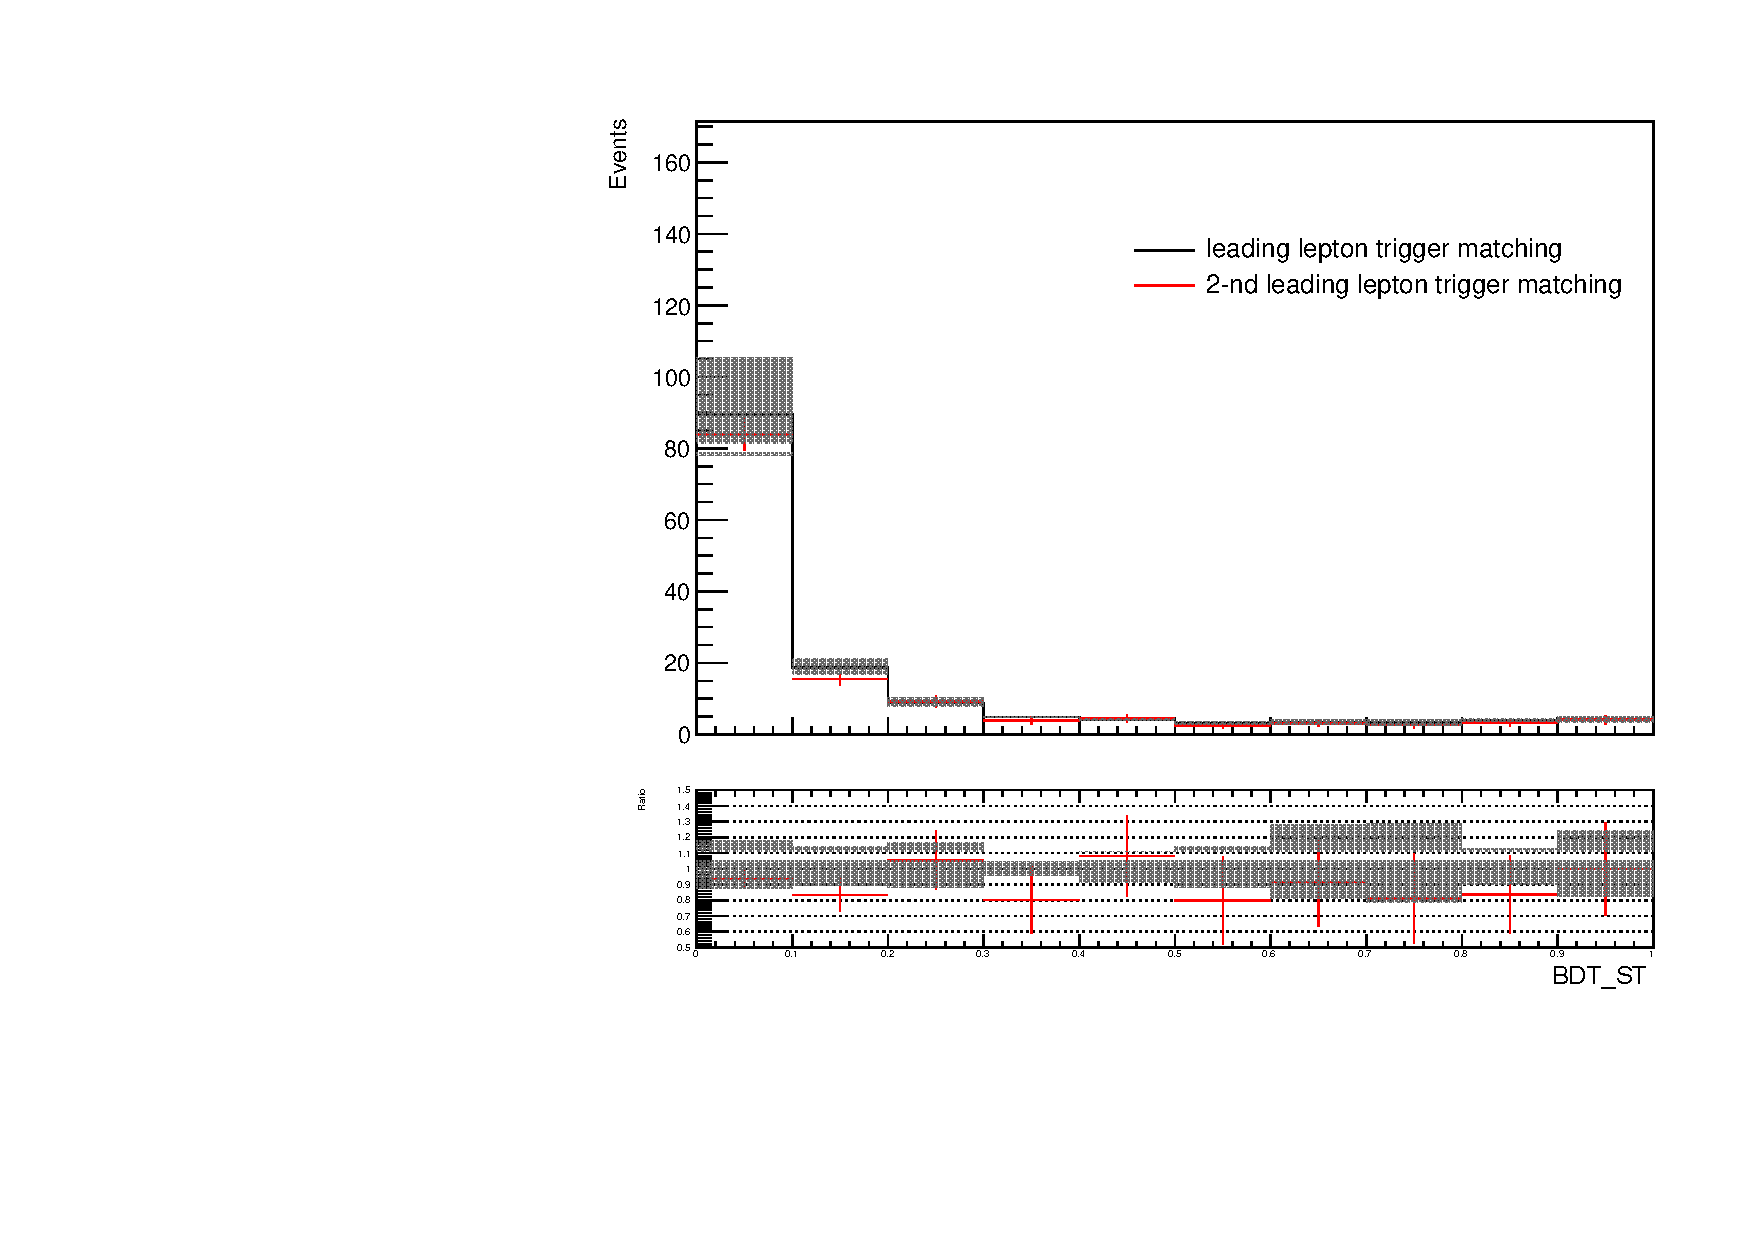
\includegraphics[width=0.47\textwidth]{figures/Part3/Systematics/BDT_ST_MM}&
 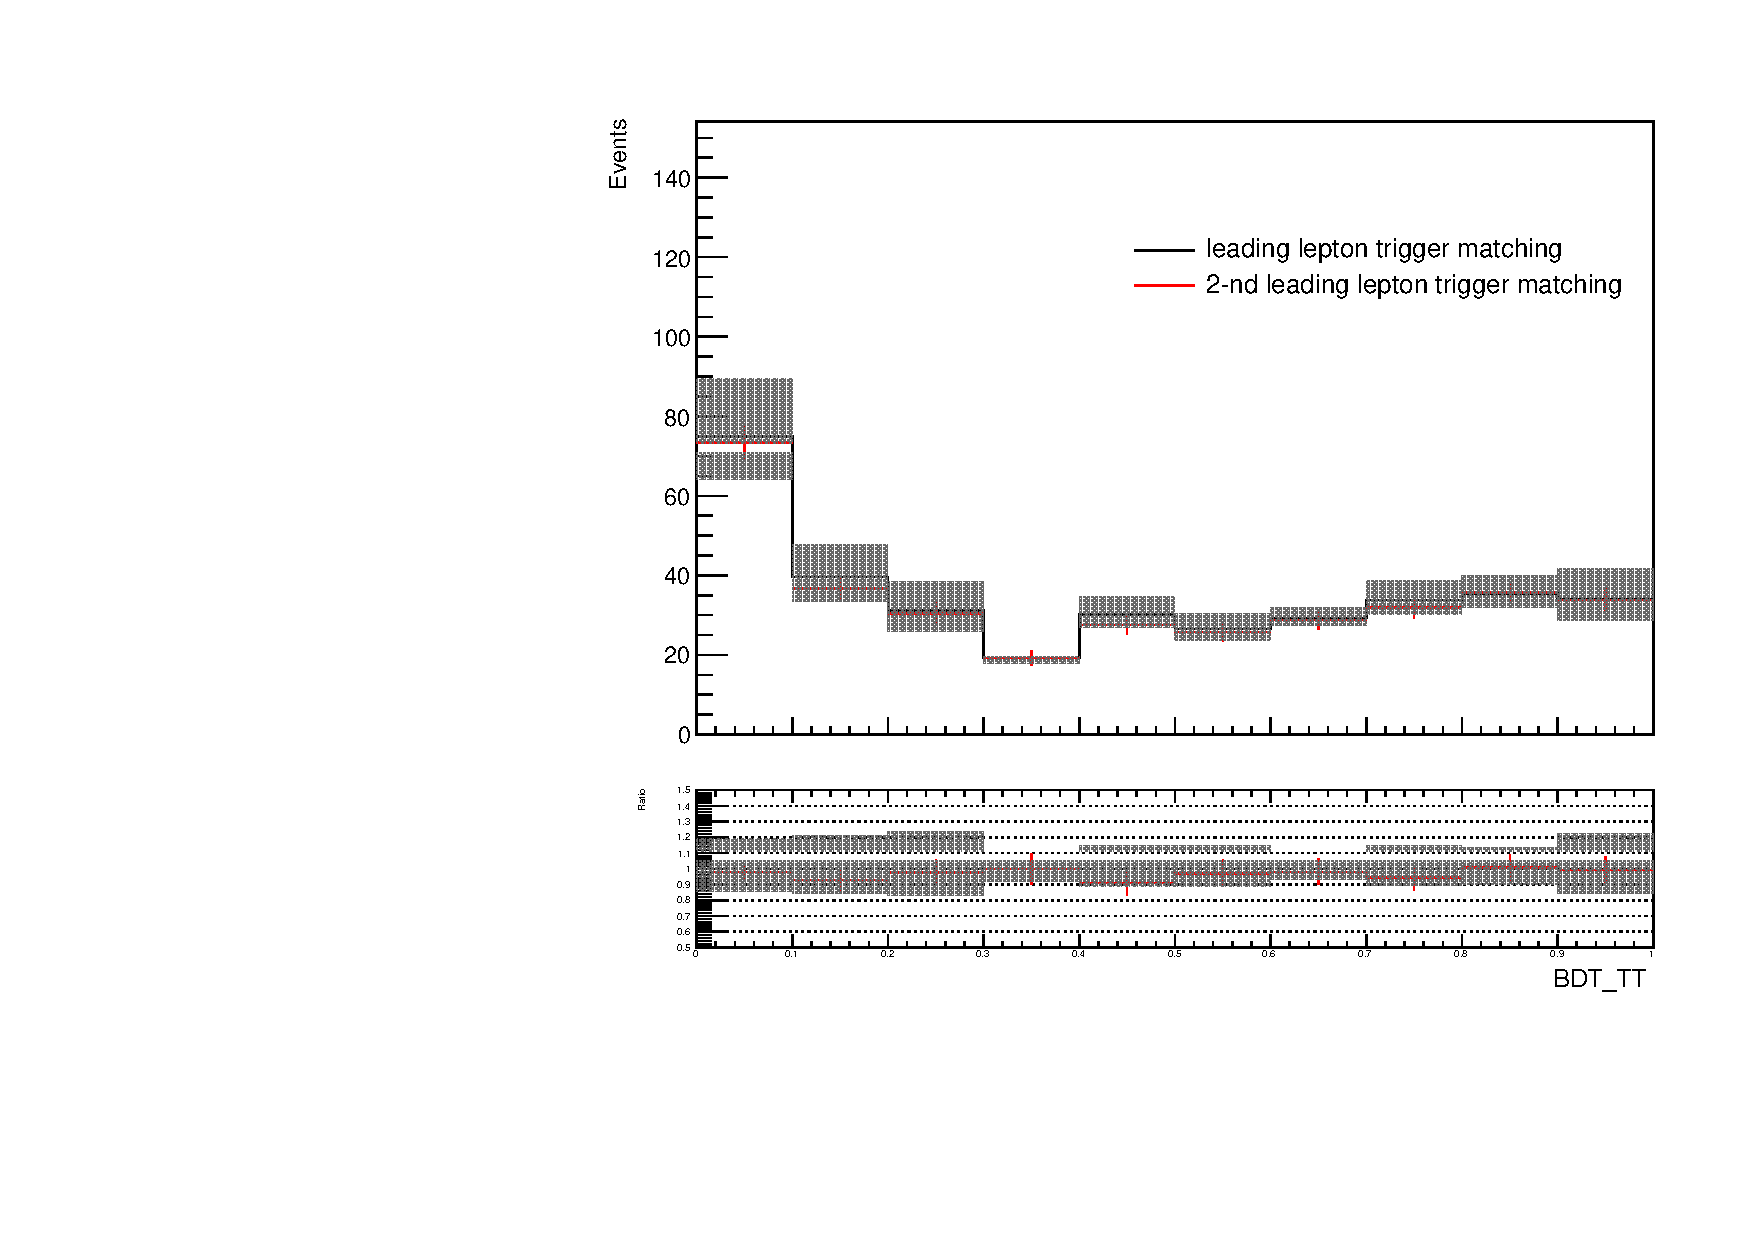
\includegraphics[width=0.47\textwidth]{figures/Part3/Systematics/BDT_TT_MM} \\
 \end{tabular}
 \caption{The impact of matching leptons to trigger objects on \emph{nonprompt} estimate. From left to right: \emph{nonprompt} estimate in top production enriched \ac{SR}, \emph{nonprompt} estimate in top decay enriched \ac{SR}. The nominal configuration of the \mm~is to match the leading lepton with trigger objects. Matching the sub-leading with the trigger objects is taken as an alternative to evaluating the robustness of the \emph{nonprompt} estimate. The uncertainty band only covers the variation of the \emph{nonprompt} estimate as a result of varying leading lepton $f$ by 50 $\%$. Uncertainty bars only include statistical uncertainties.}
 \label{fig:MM_trigger}
 \end{center}
\end{figure}

The five components of the uncertainties discussed in this section are propagated through the matrix inversion. The resulting variations of the \emph{nonprompt} estimates are taken as the uncertainties, which contain both normalization and differential effects to the \ac{BDT} templates. These uncertainties are treated uncorrelated between different components but correlated across the years. In addition to these five uncertainties, an overall normalization uncertainty of 10$\%$ is assigned to cover any other potential variations of the \emph{nonprompt} backgrounds.
%%%%%%%%%%%%%%%%%%%%%%%%%%%%%%%%%%%%%%%%%%%%%%%%%%%%%%%%
%%%%%%%%%%%%%%%%%%%%%%%%%%%%%%%%%%%%%%%%%%%%%%%%%%%%%%%%

\section{Diboson Uncertainties}
\label{sec:DiUnc}

Mismodeling of the jet multiplicity is observed in WZ control region, as is shown in Figure~\ref{fig:WZ}. This is largely due to the fact WZ process is modeled at \ac{LO} with one extra parton in the \ac{ME}. Any other extra jets are modeled by the parton shower, which is suboptimal when compared to the modeling from \ac{ME}. To take this into account, a dedicated jet-dependent uncertainty is assigned to each event. This uncertainty is determined using diboson \ac{VR} that has the same OnZ requirement as the WZ \ac{VR}, no jet multiplicity requirement, a \ac{MET} $>$ 85 GeV requirement, and a requirement of no b-tagged jets with $\pt$ $>$ 20 GeV. Unlike for the WZ \ac{VR}, events with different lepton flavor compositions are combined.

The jet multiplicity distributions in diboson \ac{VR} are shown in Figure~\ref{fig:VV_CR}. For each year, a scale factor parameterized as bins of jet multiplicity is derived,

\begin{equation}
\epsilon=\frac{N_{data}-N_{\textsf{VVV}}-N_{\textsf{t}\overline{\textsf{t}}+\textsf{X(X)}}-N_{\ttbar}-N_{others}}{N_{\textsf{VV}}}.
\end{equation}

\begin{figure}[tbh!]
 \begin{center}
 \begin{tabular}{ccc}
 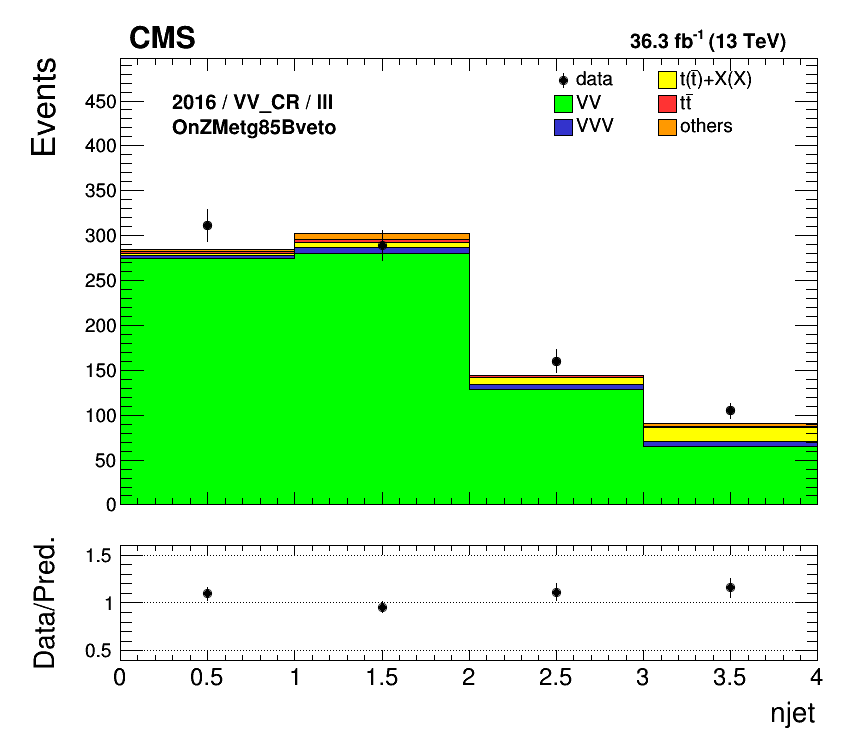
\includegraphics[width=0.325\textwidth]{figures/Part3/Systematics/njet_2016}&
  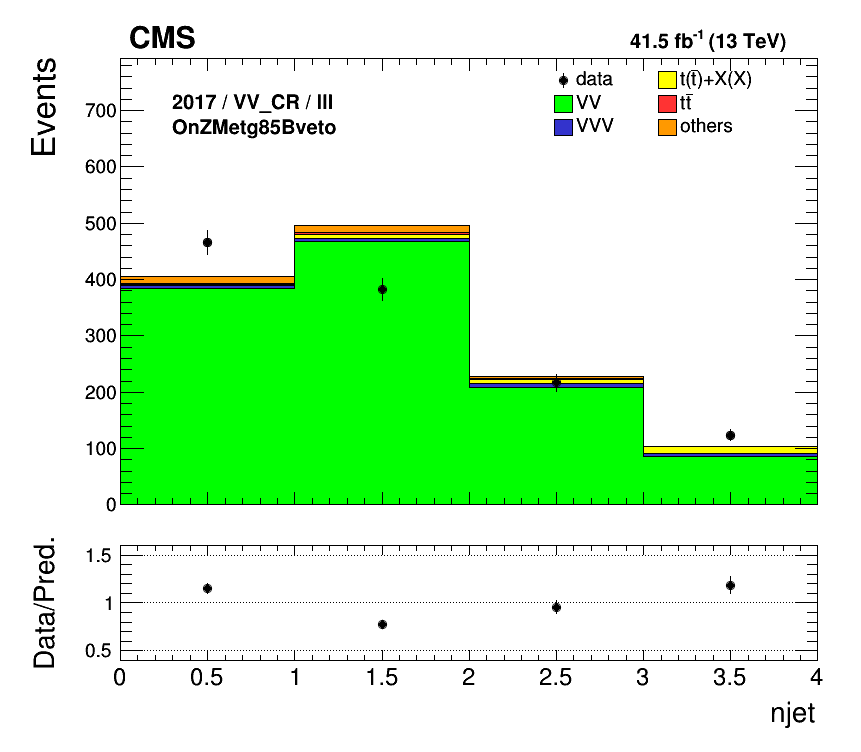
\includegraphics[width=0.325\textwidth]{figures/Part3/Systematics/njet_2017}&
 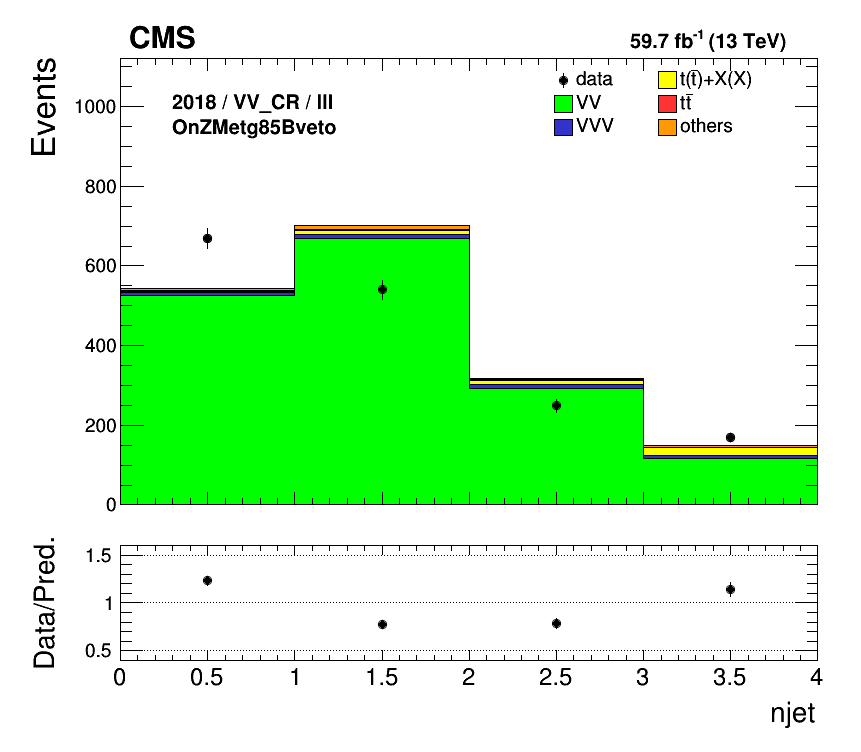
\includegraphics[width=0.325\textwidth]{figures/Part3/Systematics/njet_2018}\\
 \end{tabular}
 \caption{Distributions of the jet multiplicity in the diboson \acp{VR} in the 2016 (left), 2017 (middle) and 2018 (left) datasets. Events are required to contain exactly three \emph{tight} leptons with any composition of flavors. ``VV'' denotes the WZ and ZZ processes.}
 \label{fig:VV_CR}
 \end{center}
\end{figure}

The scale factor $\epsilon$ is used to estimate the uncertainty, denoted by $\mathrm{\Delta}$,

\begin{equation}
\mathrm{\Delta}=|1-\epsilon|
\end{equation}

\begin{figure}[tbh!]
 \begin{center}
 \begin{tabular}{ccc}
 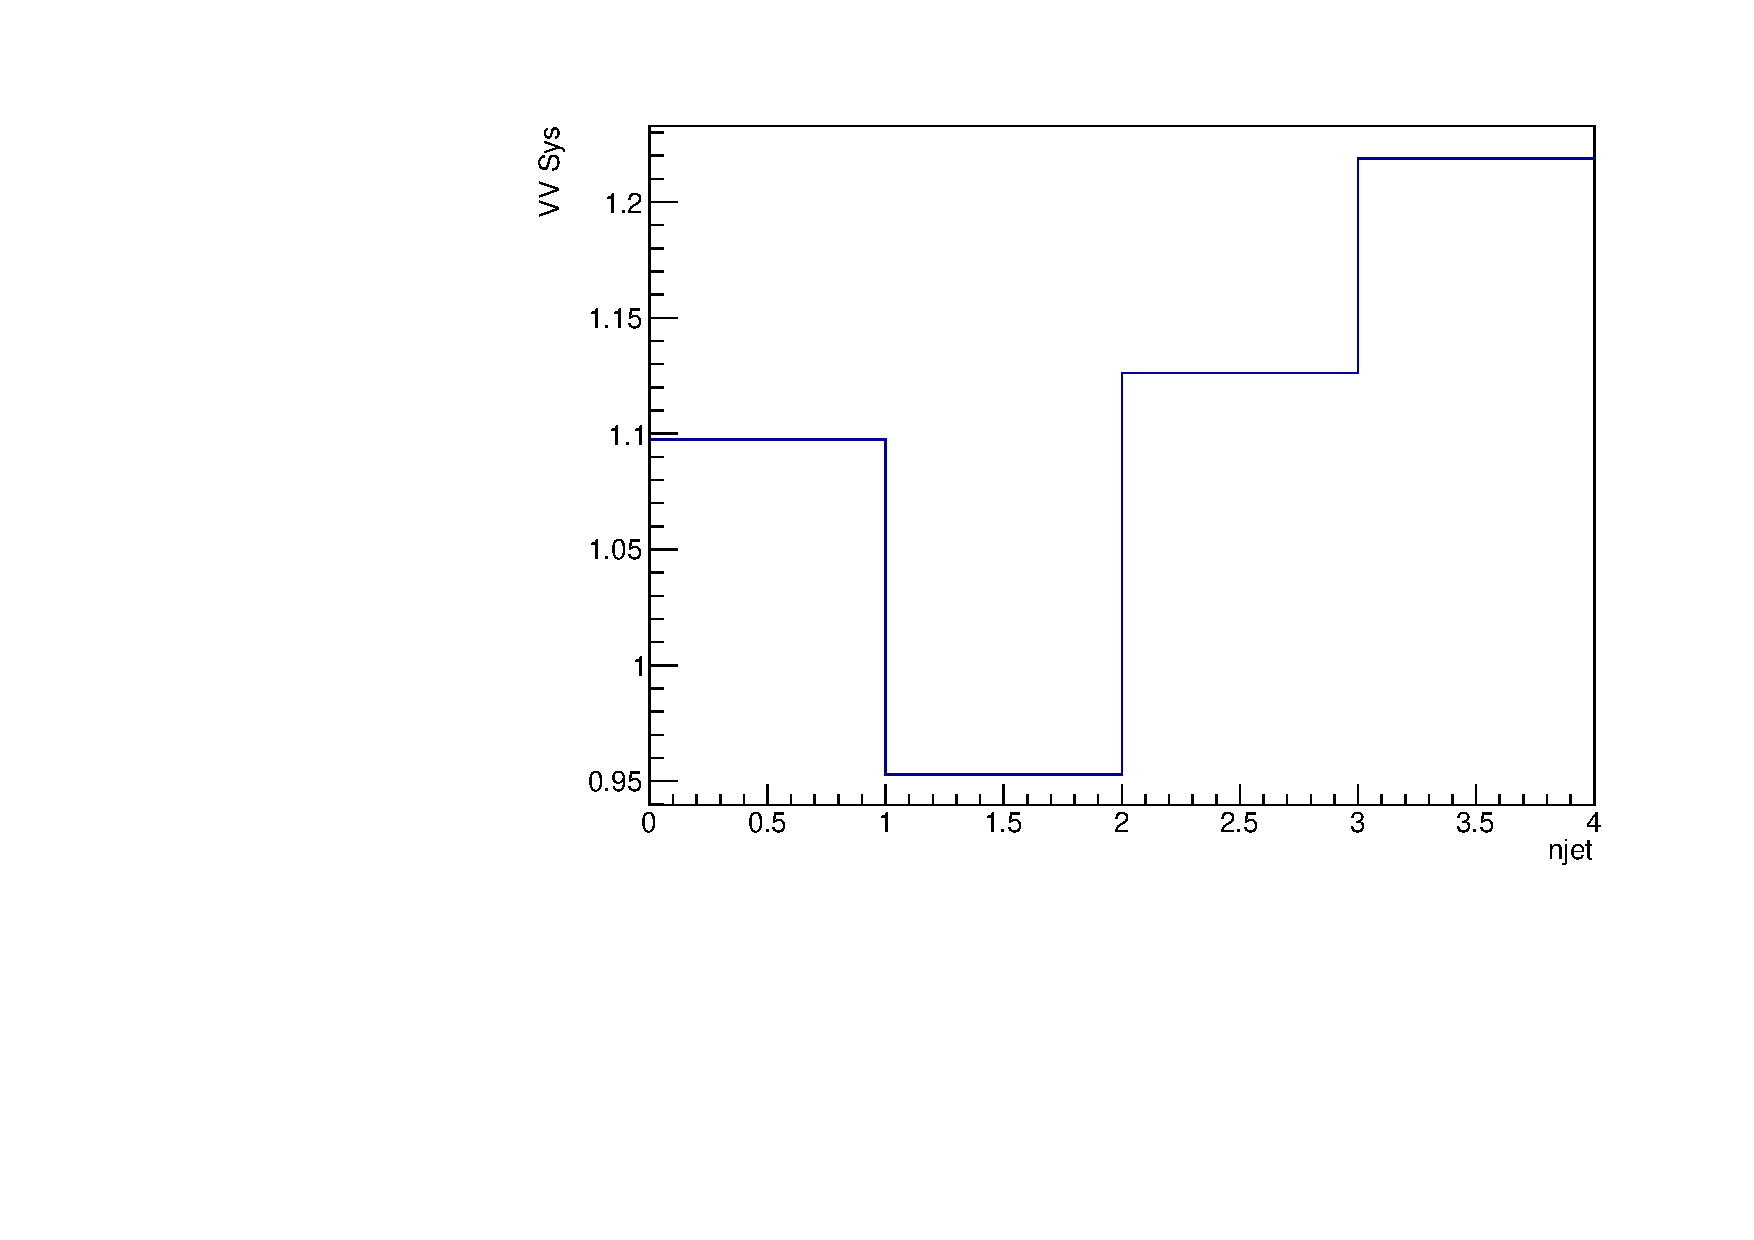
\includegraphics[width=0.325\textwidth]{figures/Part3/Systematics/2016_VV_Sys_1D}&
  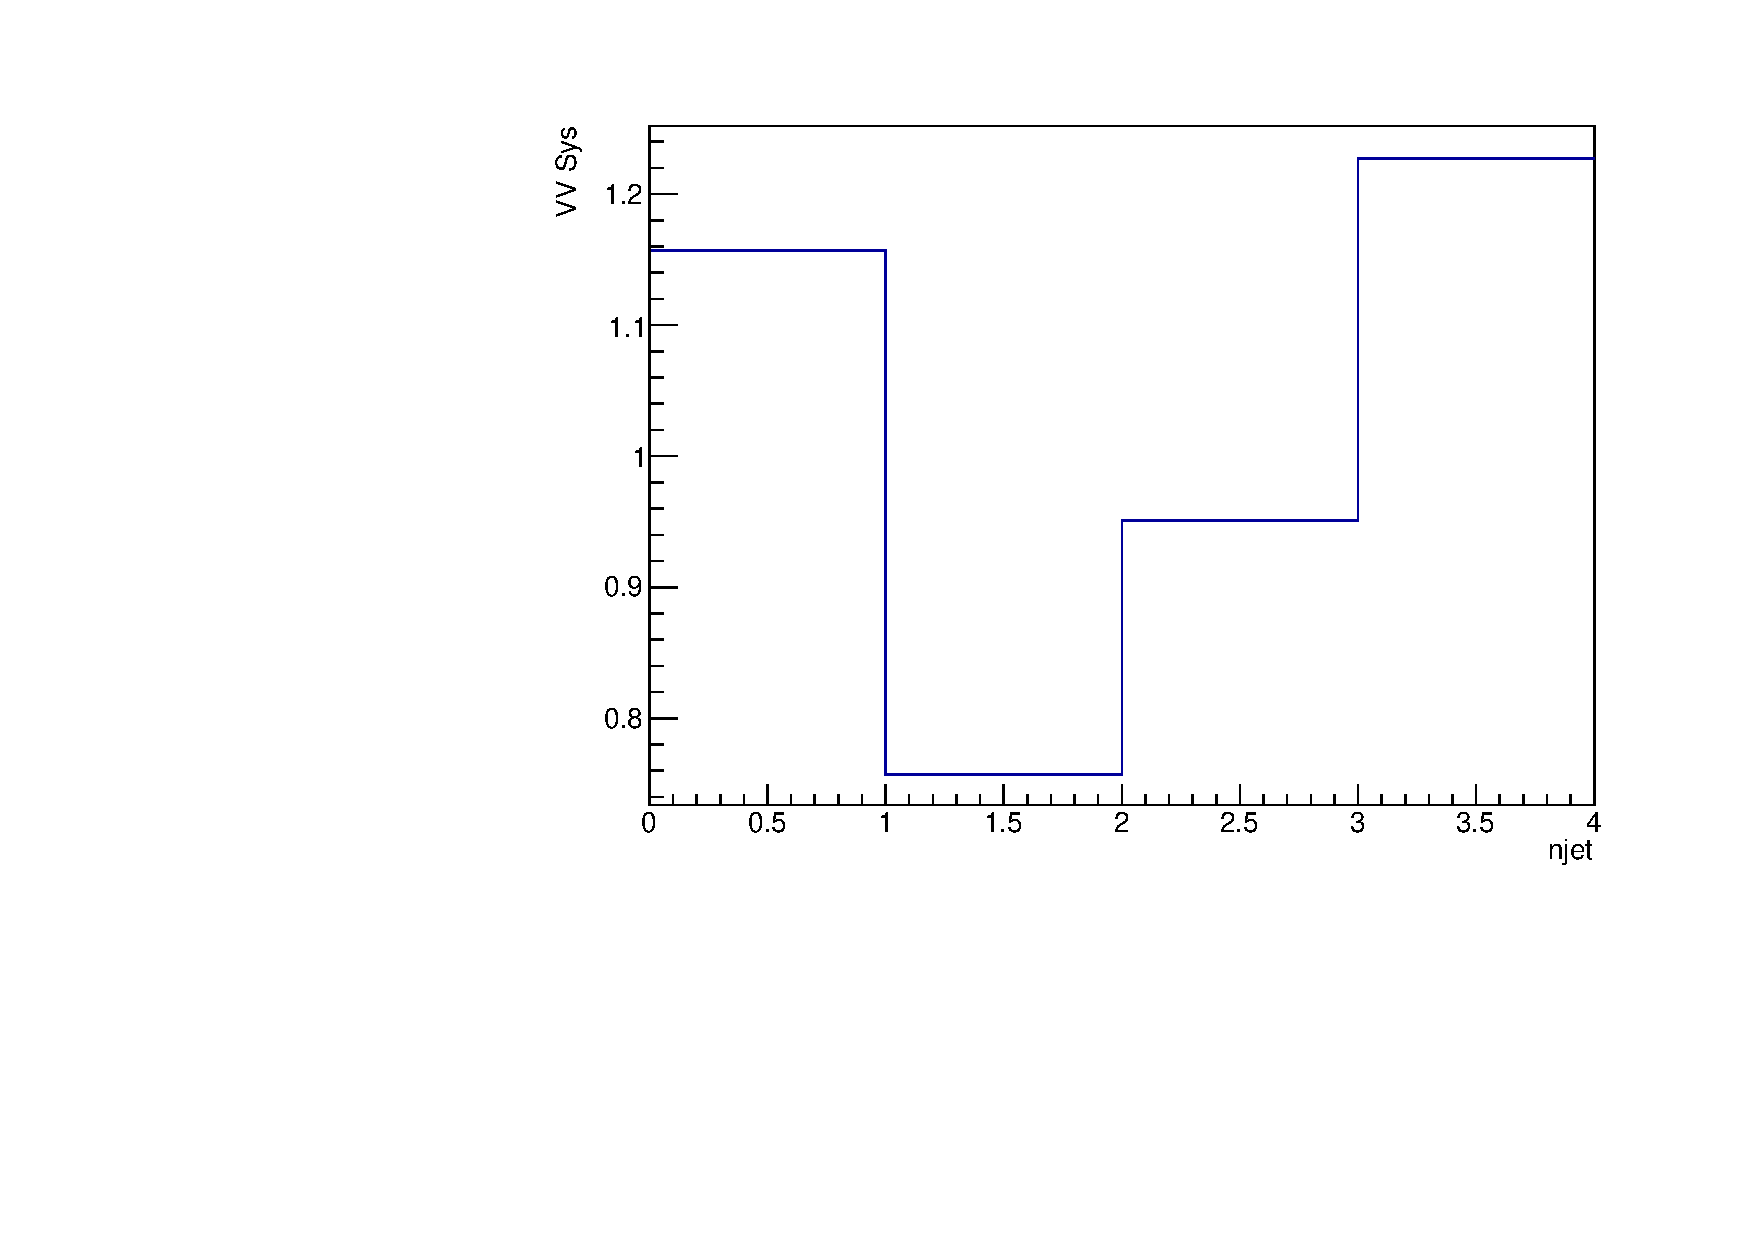
\includegraphics[width=0.325\textwidth]{figures/Part3/Systematics/2017_VV_Sys_1D}&
 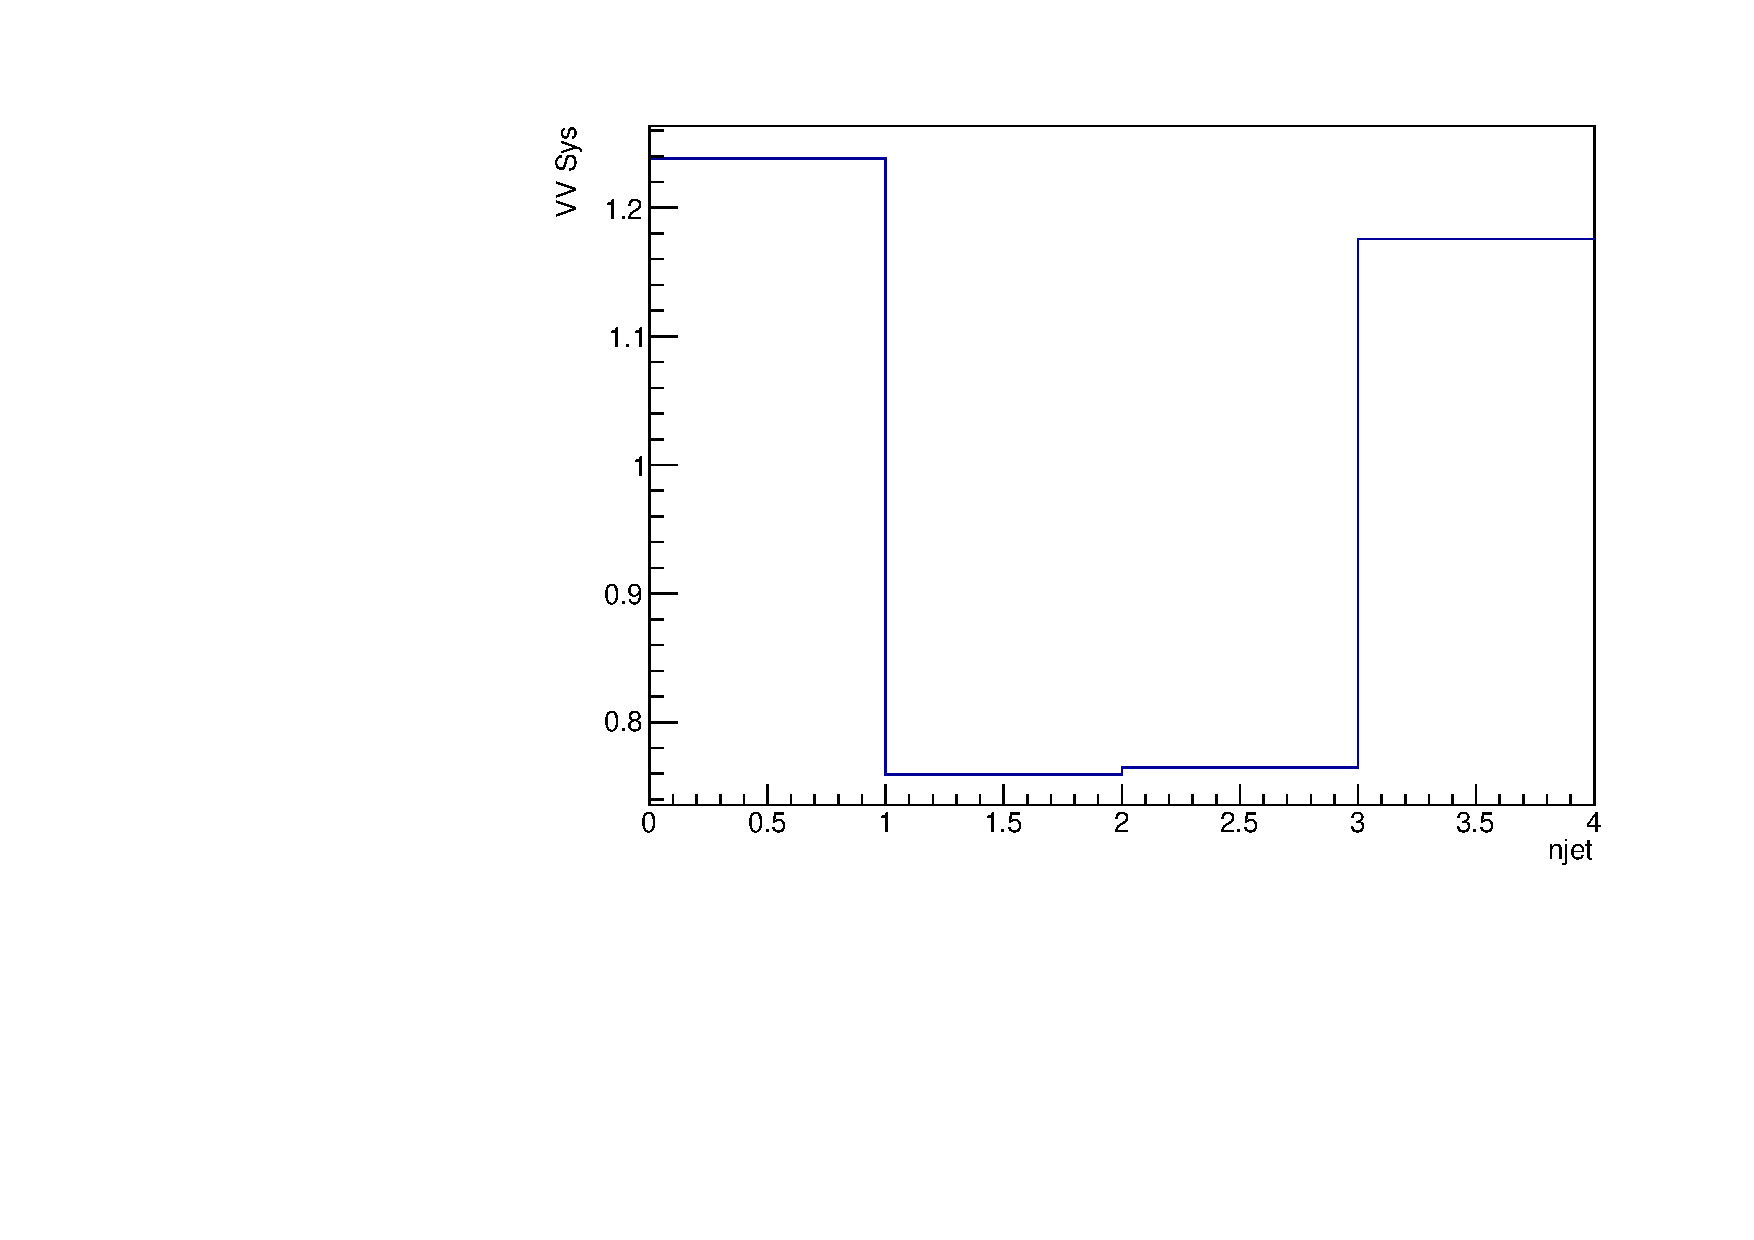
\includegraphics[width=0.325\textwidth]{figures/Part3/Systematics/2018_VV_Sys_1D}\\
 \end{tabular}
 \caption{Scale factors derived from the diboson \acp{VR} in the 2016 (left), 2017 (middle) and 2018 (right) datasets. These scale factors are used to assign uncertainties instead of correcting simulated events.}
 \label{fig:SF_VV}
 \end{center}
\end{figure}

This uncertainty modifies the predictions of WZ and ZZ processes by up to 20$\%$, as is shown in Figure \ref{fig:SF_VV}.
%%%%%%%%%%%%%%%%%%%%%%%%%%%%%%%%%%%%%%%%%%%%%%%%%%%%%%%%
%%%%%%%%%%%%%%%%%%%%%%%%%%%%%%%%%%%%%%%%%%%%%%%%%%%%%%%%

\section{Other Experimental Uncertainties}
\label{sec:OthUnc}

Uncertainties of 1.2, 2.3, and 2.5\% are assigned to the integrated luminosity for 2016, 2017, and 2018, respectively~\cite{CMS:2021xjt,CMS-LUM-17-004,CMS-LUM-18-002}. These uncertainties affect the normalization of the \ac{BDT} templates of all signals as well as \emph{prompt} backgrounds. The correlation between these uncertainties is taken into account when combining the 2016-2018 datasets. 

\ac{PU} distributions of all signals and \emph{prompt} backgrounds are reweighted using per-event scale factors to recreate the \ac{PU} profile measured in data. The uncertainties associated with these scale factors are evaluated by varying the inelastic pp cross-section by $\pm$4.6\%~\cite{Sirunyan:2018nqx}. These uncertainties are considered correlated across the years.

Calibrations of the reconstruction of electrons and muons are done centrally at \ac{CMS} by using a ``tag-and-probe'' approach~\cite{CMS:2010svw} in \ac{DY} enriched dilepton events. Per-object scale factors are used to correct for the discrepancy between reconstruction efficiencies measured in data and \ac{MC}. Limited sample size as well as the choice of fit models contribute to the uncertainties associated with these scale factors. These uncertainties are considered correlated across the years.

The \TOP covers both identification and isolation of \emph{prompt} leptons. Similar to lepton reconstruction, the calibration of \TOP is done using a tag-and-probe approach in \ac{DY} enriched dilepton events. Per-object scale factors are used to correct for the discrepancy between reconstruction efficiencies measured in data and \ac{MC}. Uncertainties of these scale factors are divided into two separate uncertainties: the statistical components of these uncertainties are treated as uncorrelated across the years while the other components are merged and treated as fully correlated across the years. For high $\pt$ electrons and muons ($\pt~>$ 200 GeV), an additional uncertainty, denoted by ``eleIDHighPt/muIDHighPt'', is assigned and it increases linearly from 0 to 10$\%$ (200 GeV-1000 GeV) and is capped at $10\%$ after 1000 GeV. These additional uncertainties are introduced because the efficiency calibration is largely done in low $\pt$ phase space. This additional uncertainty is considered correlated across the years.

Calibrations of energy scale and resolution of electrons are done centrally at CMS~\cite{CMS:2013lxn} and no uncertainties are considered as they are largely negligible. Calibrations of muon energy scale and resolution are done using the ``Rochester algorithm''~\cite{Bodek:2012id} for muons with $\pt~<$ 200 GeV. ``MuonScale'' is used to denote the uncertainties associated with this correction, which comes primarily from a limited sample size. For muons with $\pt~>$ 200 GeV, no corrections are applied as there are not enough events for a robust correction from the ``Rochester algorithm''. An additional uncertainty, also denoted by ``MuonScale'' is assigned to the momentum of these high $\pt$ muons using the ``Generalized Endpoint method''~\cite{CMS:2018rym}. The ``MuonScale'' uncertainty is considered correlated across the years.

No calibration is done for trigger efficiency as they are generally close to 1 in both data and \ac{MC}. A flat 2$\%$ uncertainty is assigned to all signals and \emph{prompt} backgrounds to cover statistical fluctuations. This uncertainty is treated as uncorrelated across the years.

Calibrations of the \DeepJ scores are described in \autoref{sec:Jets}. Uncertainties associated with the calibrations are divided into 8 different sources to properly account for the correlations, which are summarized in Table~\ref{tab:btagsys}. For b and udsg jets, lf, hf, hfstats1/2, and lfstats1/2 uncertainties are applied. For c jets, cferr1/2 uncertainties are applied. 

\begin{table}[!hbtp]
\sffamily
\centering
\caption{
Summary of the sources of uncertainties associated with the b-tagging calibration, excluding those originate from \ac{JES} and \ac{JER}. A hyphen ($-$) denotes that a source is not correlated across the years.
}
\begin{tabular}{lcl}
\toprule
Source & Correlated & Description\\
\midrule
lf			& \checkmark & udsg+c jets in heavy flavor region\\ %HF$^1$
hf			& \checkmark & b+c jets in light flavor region \\ %LF$^2$
hfstats1	& - 		 & Linear fluctuations of c jets\\
hfstats2	& -			 & Quadratic fluctuations of c jets \\
lfstats1	& -			 & Linear fluctuations of udsg jets \\
lfstats2	& -			 & Quadratic fluctuations of udsg jets \\
cferr1		& \checkmark & Linear fluctuations of c jets \\
cferr2		& \checkmark & Quadratic fluctuations of c jets \\
\bottomrule
\end{tabular}
\label{tab:btagsys}
\end{table}

Calibrations of \ac{JES} and \ac{JER} are done centrally at \ac{CMS}~\cite{CMS:2016lmd}. Uncertainties associated with the \ac{JES} calibrations are divided into 27 sources to properly account for correlations, which are summarized in Table~\ref{tab:jec}. Uncertainties associated with the calibrations of \ac{JER} are combined into a separate uncertainty, which is considered uncorrelated across the years. Variations of \ac{JES} and \ac{JER} due to these uncertainties are propagated to the \ac{MET} and calibrations of the \DeepJ scores: scale factors used to correct \DeepJ scores and the \ac{MET} vector are recomputed for each of the jet energy variations and treated as uncertainties that are fully correlated to the respective jet energy variation. 

\begin{table}[!hbtp]
\sffamily
\centering
\caption{
Summary of the sources of uncertainty associated with \ac{JES}. A hyphen ($-$) denotes that a source is not correlated across the years.
}
\label{tab:jec}
\begin{tabular}{lc|lc}
\toprule
Source & Correlated & Source & Correlated \\
\midrule
AbsoluteStat			& -		&	 RelativePtHF			& \checkmark			 \\
AbsoluteScale			& \checkmark		&	 RelativeBal				& \checkmark			 \\
AbsoluteMPFBias			& \checkmark 	&	 RelativeSample			& -			 \\	 
Fragmentation			& \checkmark		&	 RelativeFSR				& -			 \\
SinglePionECAL			& \checkmark	&	 RelativeStatFSR			& \checkmark			 \\	 
SinglePionHCAL			& \checkmark	&	 RelativeStatEC			& -			 \\	 
FlavorQCD				& \checkmark	&	 RelativeStatHF			& -			 \\	 
TimePtEta				& -			 &     PileUpDataMC			& \checkmark			 \\
RelativeJEREC1			& -		&	  PileUpPtRef				& \checkmark			 \\
RelativeJEREC2			& -		&	  PileUpPtBB				& \checkmark			 \\
RelativeJERHF			& \checkmark		&	 PileUpPtEC1				& \checkmark			 \\
RelativePtBB			& \checkmark		&	 PileUpPtEC2				& \checkmark			 \\
RelativePtEC1			& -			&   PileUpPtHF				& \checkmark			 \\
RelativePtEC2			& -			&   & \\
\bottomrule
\end{tabular}
\end{table}

One additional uncertainty is assigned to the unclustered \ac{MET} is considered~\cite{CMS:2019ctu}, and is treated as uncorrelated across the years.

In the 2016 and 2017 runs, \ac{L1} ECAL triggers fired early~\cite{CMS:2020cmk} causing many uninteresting events to be recorded while the later interesting events were rejected. Since this effect is not present in the \ac{MC} simulation, a correction is applied to all signals and \emph{prompt} backgrounds. This correction is varied by 20\% and the resulting change in per-event weight is taken as the uncertainty. This uncertainty is treated as correlated across the years. 

In the 2018 runs, two HCAL modules whose power supply died in the middle of the data taking. This affected the measurement of jet energy and \ac{MET}. No correction is applied as this effect is not well-understood and likely not significant relative to other corrections. Nevertheless, an uncertainty, denoted by ``HEM'', is assigned to cover the variations of jet energy and \ac{MET} caused by those two dead modules. 

A comparison of different sources of systematic uncertainties of the background estimates in the \acp{SR} is shown in Figure~\ref{fig:Comp_sys_background}.

\begin{figure}[tbh!]
 \begin{center}
 \begin{tabular}{cc}
  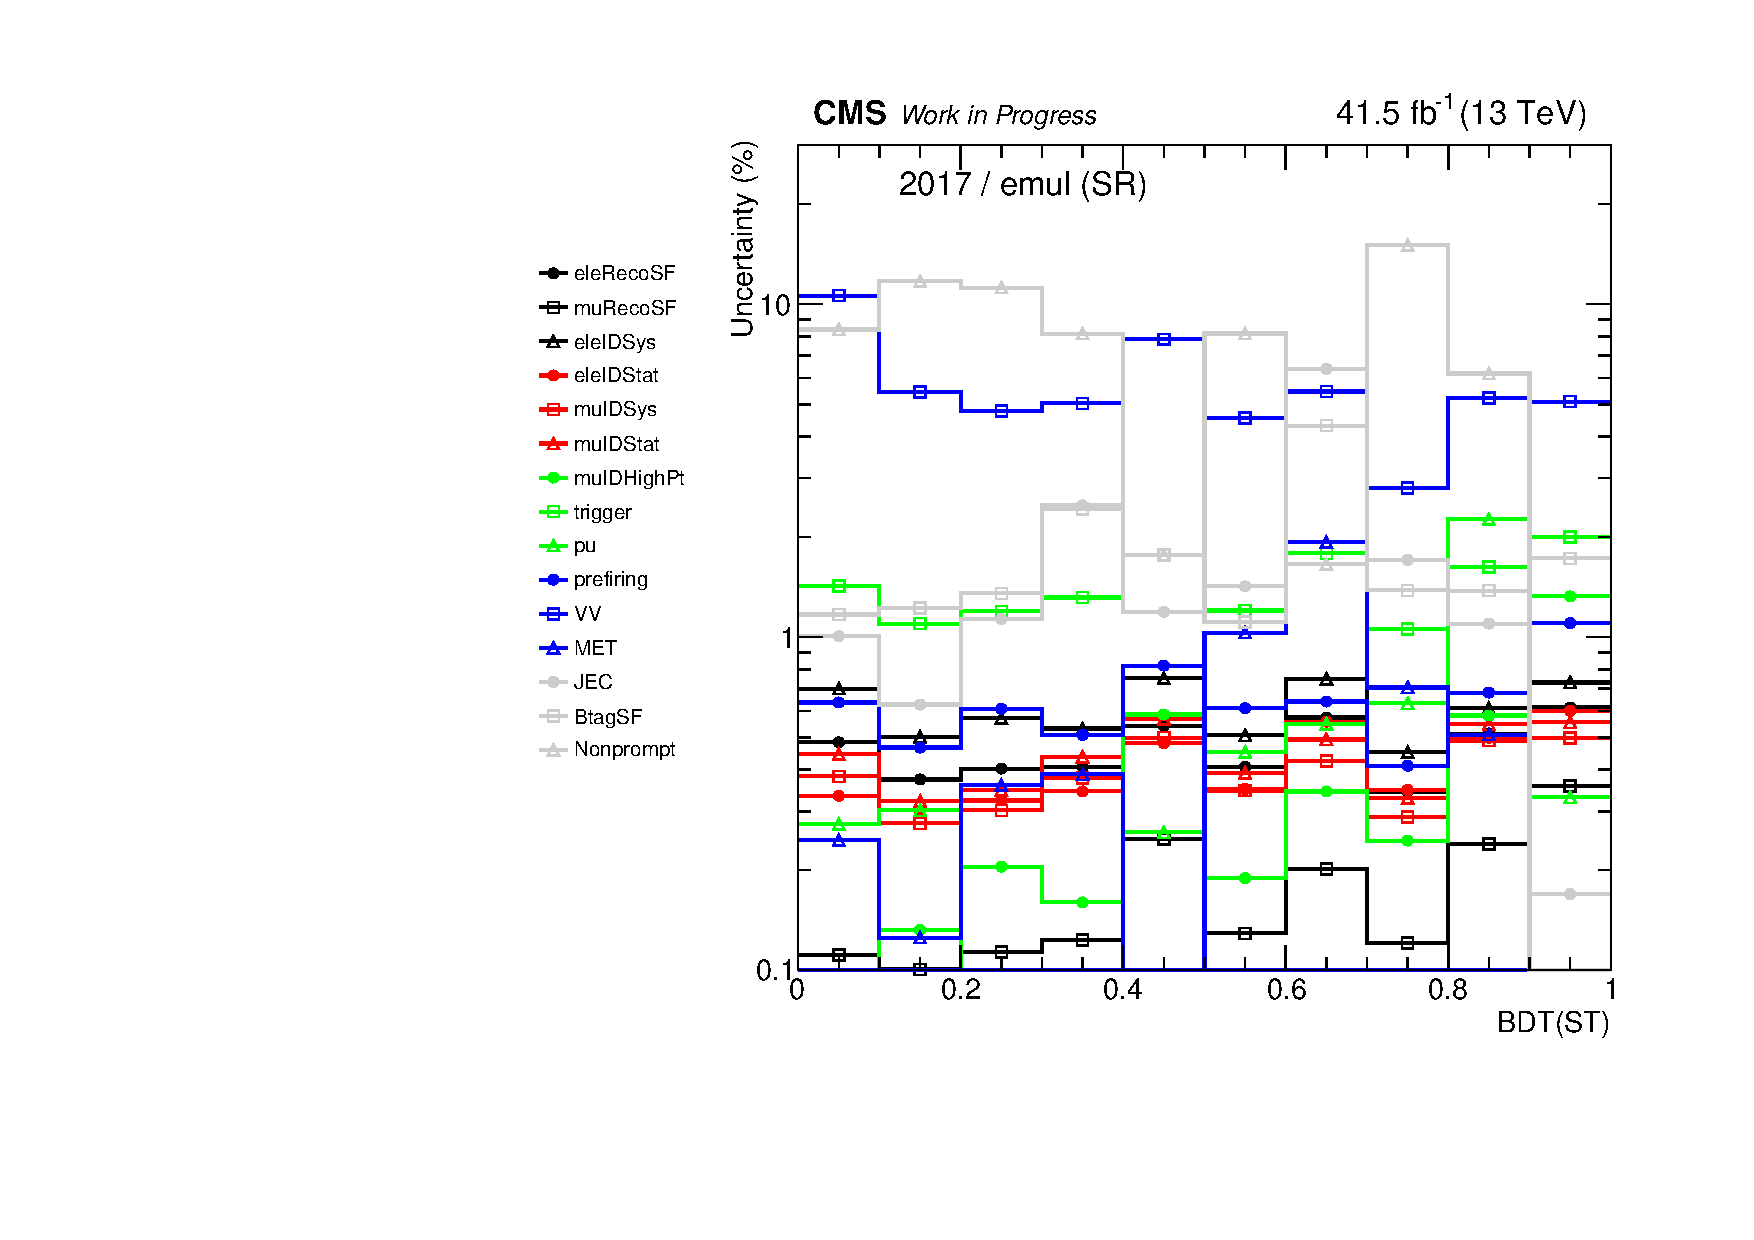
\includegraphics[width=0.45\textwidth]{figures/Part3/Systematics/sysBDT_ST_bkg_2017}&
 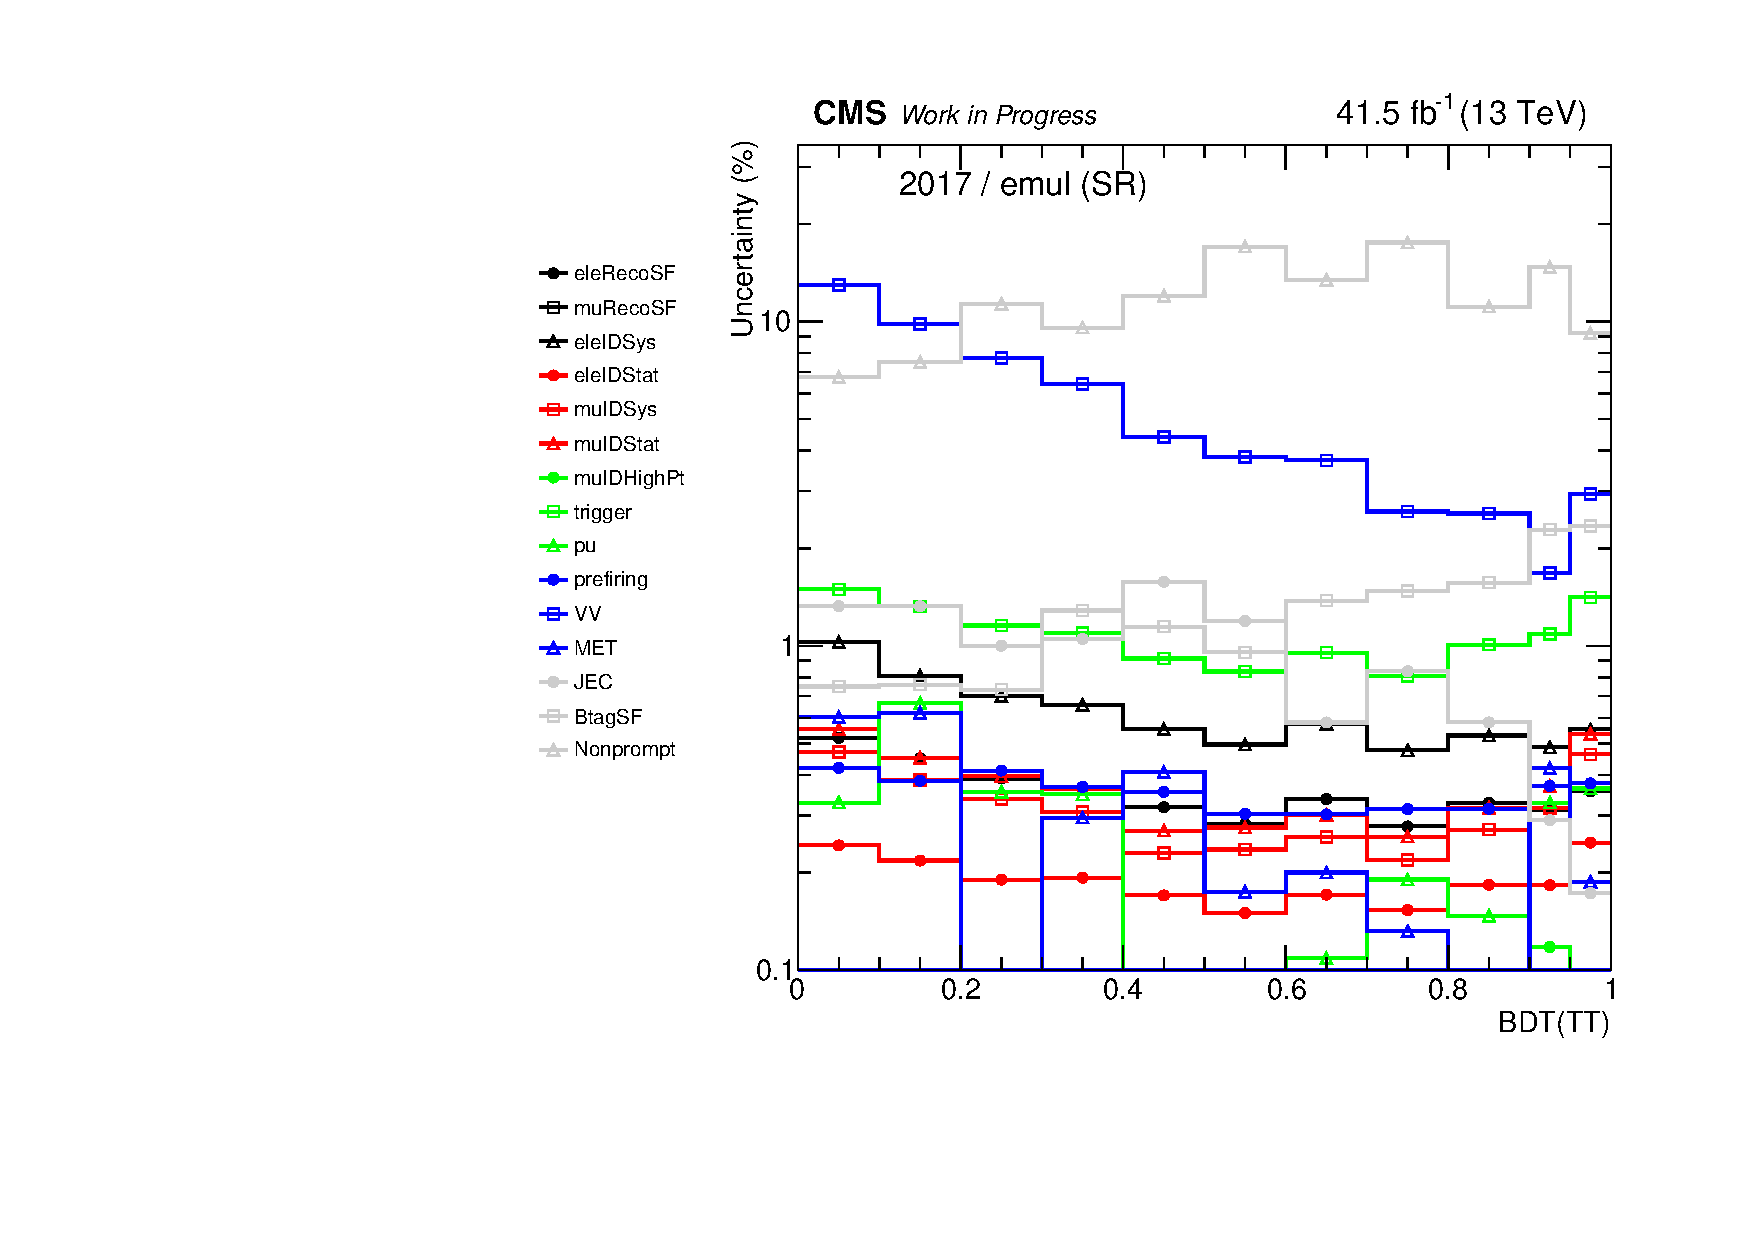
\includegraphics[width=0.45\textwidth]{figures/Part3/Systematics/sysBDT_TT_bkg_2017} \\
 \end{tabular}
 \caption{Distributions of relative uncertainties on total expected backgrounds as a function of \ac{BDT} output in top production enriched \ac{SR} (left), top decay enriched \ac{SR} (right). Luminosity and cross-section uncertainties are not included in these plots. \ac{JES}, \ac{JER}, and HEM are combined into ``JEC''. Sources of b-tagging uncertainties listed in Table~\ref{tab:btagsys} are combined into ``BtagSF''.}
 \label{fig:Comp_sys_background}
 \end{center}
\end{figure}

A comparison of different sources of systematic uncertainties of the signal estimates in the \acp{SR} is shown in Figure~\ref{fig:Comp_sys_signal}.

\begin{figure}[tbh!]
 \begin{center}
 \begin{tabular}{cc}
  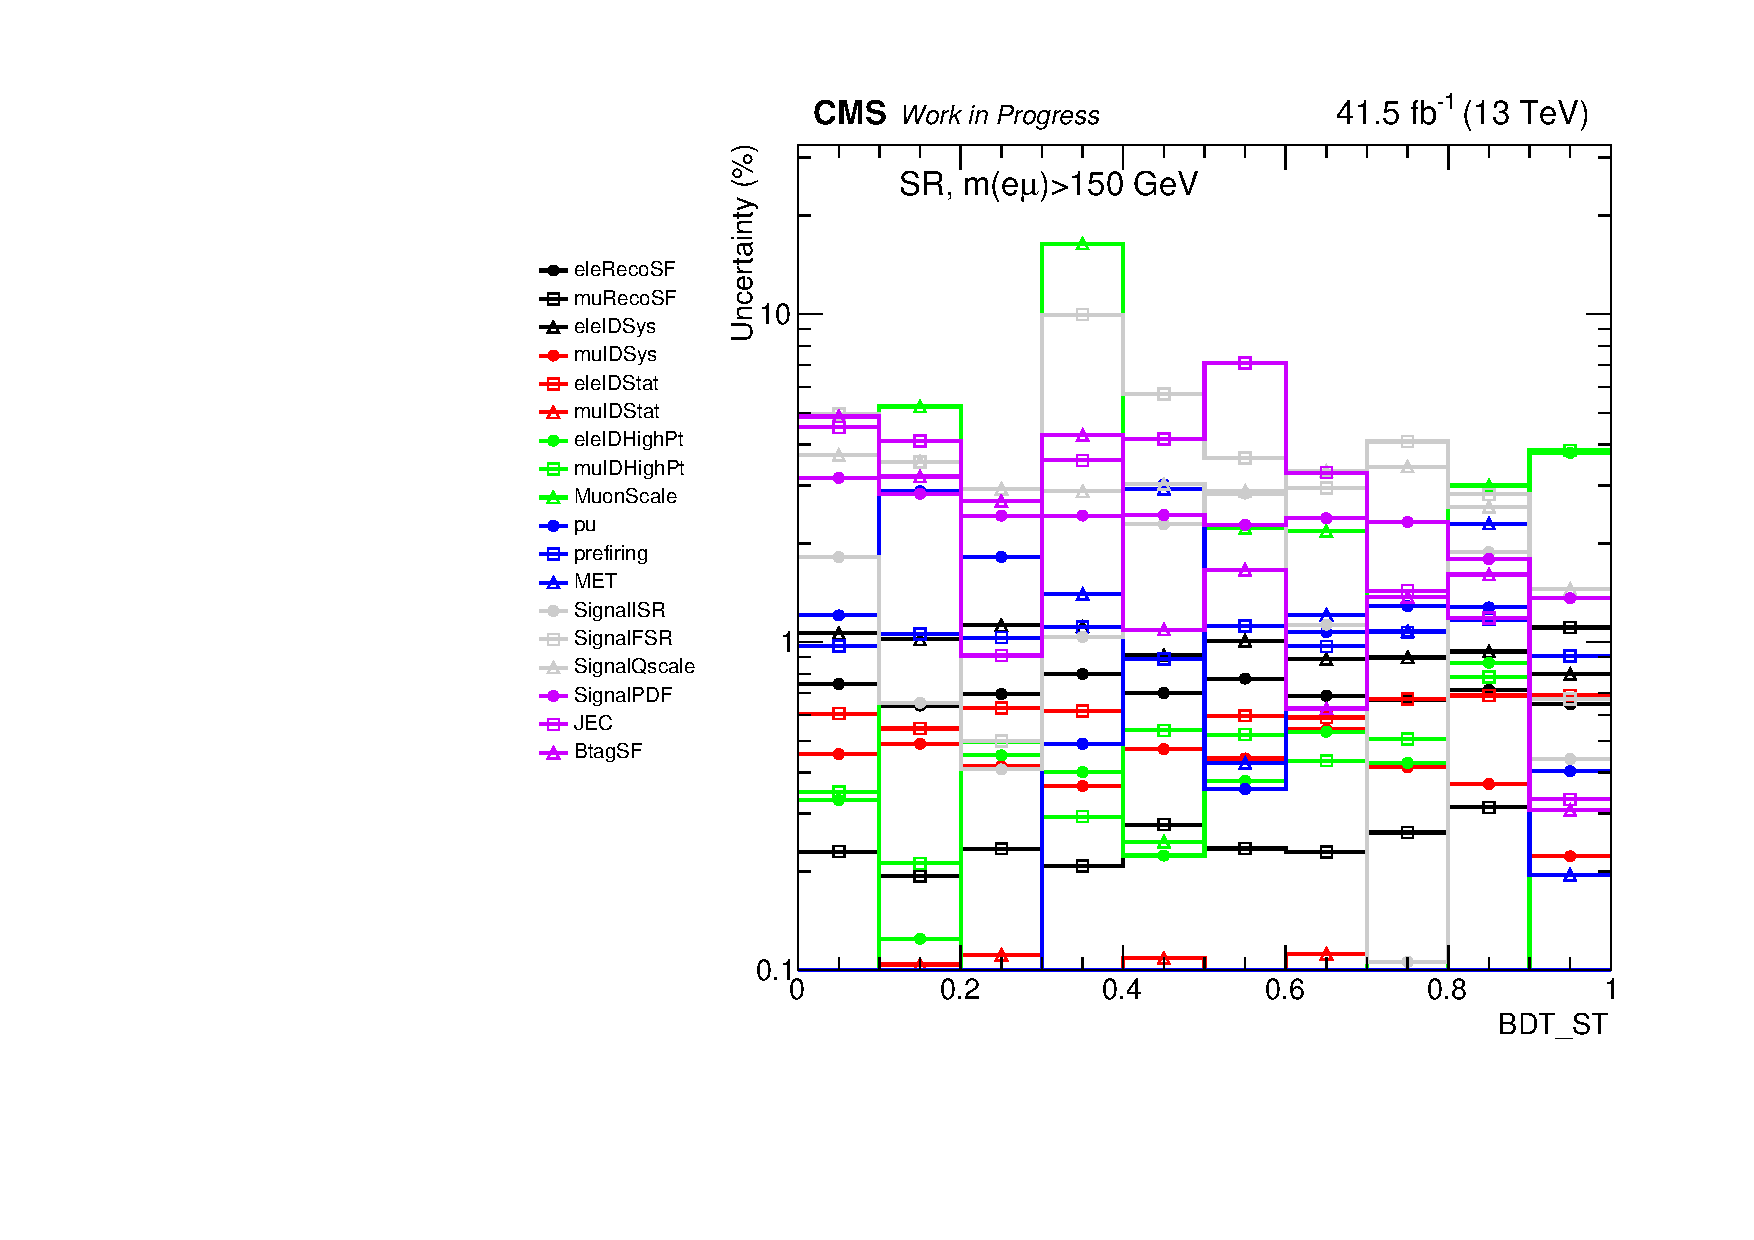
\includegraphics[width=0.45\textwidth]{figures/Part3/Systematics/sysBDT_ST_sig_2017}&
 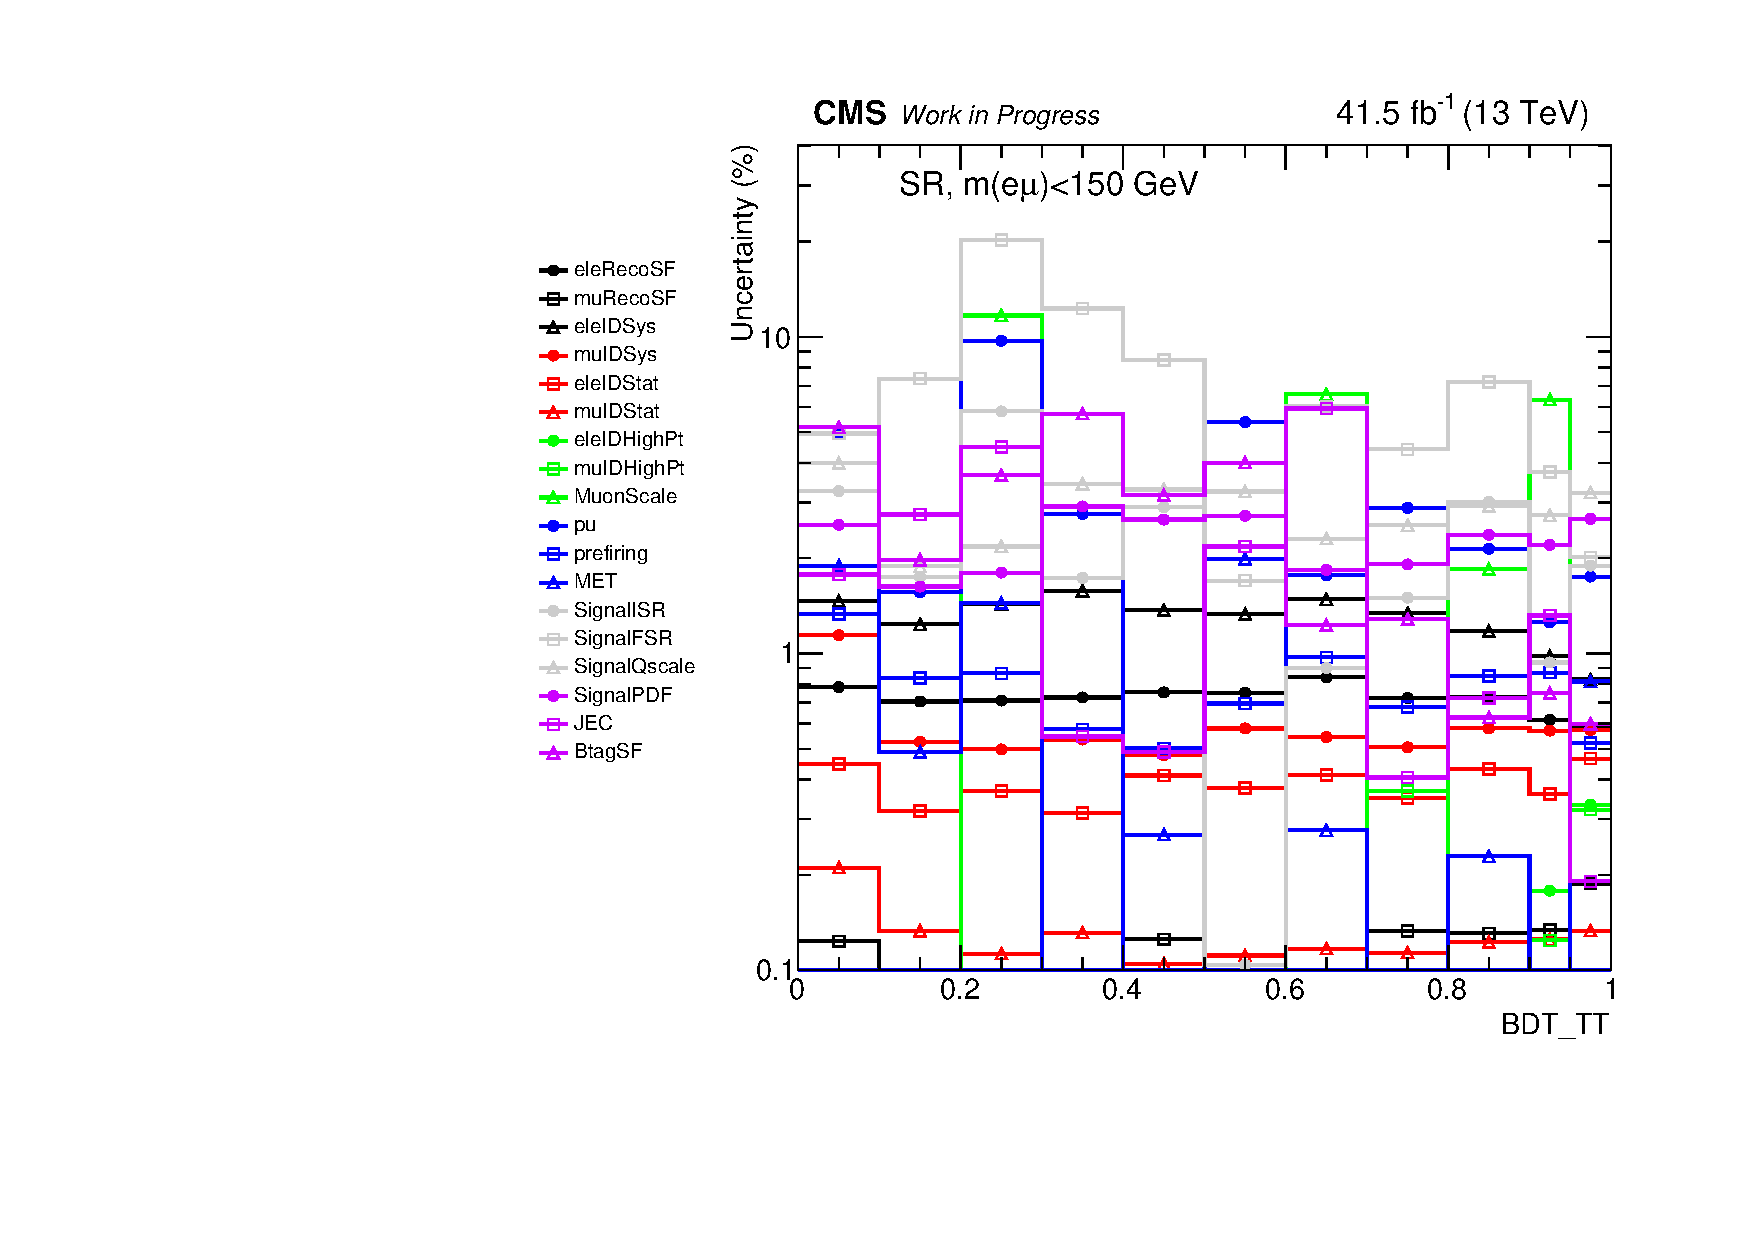
\includegraphics[width=0.45\textwidth]{figures/Part3/Systematics/sysBDT_TT_sig_2017} \\
 \end{tabular}
 \caption{Distributions of relative uncertainties on signal ($\WC{\textsf{vector}}{\emut{u}}$ is used as an example) as a function of \ac{BDT} output in top production enriched \ac{SR} (left), top decay enriched \ac{SR} (right). Luminosity and cross-section uncertainties are not included in these plots. \ac{JES}, \ac{JER}, and HEM are combined into ``JEC''. Sources of b-tagging uncertainties listed in Table~\ref{tab:btagsys} are combined into ``BtagSF''.}
 \label{fig:Comp_sys_signal}
 \end{center}
\end{figure}

A summary of systematic uncertainties and their average impact on predicted yields in the \acp{SR} can be found in Table~\ref{tab:repsys}. These uncertainties are extracted from pre-fit \ac{BDT} templates shown in Figure~\ref{fig:bdt_output}.

\begin{table}[th]
\sffamily
\centering
\caption{Summary of systematic uncertainties and the average change in signal and overall background yields in the SRs. Uncertainties that only contain normalization effects, such as luminosity uncertainties and uncertainties on theoretical cross sections, are not included in this table.}
\resizebox{0.95\linewidth}{!}{%
\begin{tabular}{ccccc}
\toprule
\multirow{2}{*}{Systematic uncertainty} & \multicolumn{2}{c}{$\memu~<~150$ GeV} & \multicolumn{2}{c}{$\memu~>~150$ GeV} \\
             & Background & Signal     & Background & Signal \\
\midrule
Lepton reconstruction & $<0.1\%$ & 0.6$\%$ & $<0.1\%$ & 1.7$\%$\\
Lepton identification and isolation & 1.0$\%$ & 1.4$\%$ & 1.0$\%$ & 1.3$\%$\\
High $\pt$ lepton & $<0.1\%$ & 0.2$\%$ & $<0.1\%$ & 3.4$\%$\\
Muon momentum scale and resolution & $<0.1\%$ & 0.3$\%$ & $<0.1\%$ & 0.1$\%$\\
PDF & $<0.1\%$ & 2.3$\%$ & $<0.1\%$ & 1.3$\%$\\
QCD scale & 4.0$\%$ & 2.8$\%$ & 5$\%$ & 1.4$\%$\\
ISR/FSR & - & 7.6$\%$ & - & 1.0$\%$\\
Pileup & $<0.1\%$ & 0.4$\%$ & $<0.1\%$ & 0.3$\%$\\
L1 prefiring & $<0.1\%$ & 0.4$\%$ & $<0.1\%$ & 0.4$\%$\\
Jet energy scale and resolution& $<0.1\%$ & 1.0$\%$ & 1.0$\%$ & 0.4$\%$\\
b tagging & $<0.1\%$ & 0.9$\%$ & 1.0$\%$ & 0.5$\%$\\
Nonprompt & 11.0$\%$ & - & 9.0$\%$ & - \\
Jet modeling & 6.0$\%$ & - & 7.0$\%$ & - \\
\bottomrule
\end{tabular}
\label{tab:repsys}
}
\end{table}